\documentclass[master,euler,twoside,openright]{ustcthesis}
% 默认twoside 双面打印
% 将master修改为bachelor, doctor or master
% 要使用adobe字体,添加adobefonts选项
% 要使用Mac系统的字体,添加macfonts选项
% 使用euler数学字体,如不愿使用,去掉euler
% 使用外文写作,请添加notchinese

% 设置图形文件的搜索路径
\graphicspath{{figures/}}

%仅用于本示例文档中显示特殊字符串
\usepackage{xltxtra}
\usepackage{listings} %用listing作为代码展示的库

%%%%%%%%%%%%%%%%%%%%%%%%%%%%%%
%% 封面部分
%%%%%%%%%%%%%%%%%%%%%%%%%%%%%%

  % 中文封面内容
  \title{基于中文字符识别的\\医学档案生成与自动归类}%一般情况下扉页和封皮、书脊共用一个标题文本,可以不用定义\spinetitle(仅硕博有用), \covertitle(本硕博均有用)和\encovertitle(仅本科有用)。特殊情况见下。
  \spinetitle{\small{基于中文字符识别的医学档案生成与自动归类}}
  %\spinetitle{\small{中国科学技术大学本硕博毕业论文模板示例文档\raisebox{-3pt}{(Beta)}}}
  %特殊情况1:本例中\title命令里含有换行控制字符,这会导致制作书脊的时候出现错误,例如如果你注释掉\spinetitle{...}这一行就会报错。这时需要定义一个不含换行等命令的\spinetitle,这并不表示\spinetitle里不能有任何命令——只能使用有限的命令。
  %特殊情况2:本例中标题过长,所以需要缩小书脊标题的字号。
  %特殊情况3:本例中中英文混排,由于tex竖排的原理限制,中英文基线不重合,所以需要人工调整英文的基线。具体调整量根据不同字体有所不同。
  \covertitle{基于中文字符识别的\\医学档案生成与自动归类}
  %\covertitle{中文题目第一行\\中文题目第二行}
  %不要在此调整封皮字体大小! Do not set Cover Page font size here!
  %特殊情况4:本例中\title中含有多个换行,导致标题超过了两行。根据制本厂规定,封皮标题不能超过两行。因此需要定义封皮使用的标题\covertitle. 如果你注释掉这一行,就会发现封皮不符合规定。
  \encovertitle{USTC Thesis Template for Bachelor, Master and Doctor User's Guide(Beta)}
  %\encovertitle{English Title Line 1\\English Title Line 2\\English Title Line 3}
  %不要在此调整封皮字体大小! Do not set Cover Page font size here!
  %特殊情况5:仅本科生有用。本科封皮中有英文标题,不超过三行。与上类似。

  \author{沈汪洋}
  \depart{11系}%系别,硕博请用系代号,本科请用全称如
  %\depart{数理化和信息工程系}
  \major{计算机应用技术}%专业,硕博请用全称,本科不需要
  \advisor{唐珂\ 教授}
  %\coadvisor{冯晨珠\ 教授}%第二导师,没有请注释掉
  \studentid{SA13011913}%For bachelor only
  \submitdate{二〇一六年四月}

  % 英文封面内容
  \entitle{Automatic patients' profiles generation based on Chinese character recognition}
  \enauthor{Wangyang Shen}
  \enmajor{Computer Science}
  \enadvisor{Prof. Ke Tang}
  %\encoadvisor{Prof. Chenzhu Feng}%另外一个导师
  \ensubmitdate{April, 2016}

%%%%%%%%%%%%%%%%%%%%%%%%%%%%%%%%%%%%%%%%%%%%%%%%%%%%%%%%%%%%%%%%%%%%%
% If you use another language instead of chinese or english, then you
% should define some strings and provide information in your language.
%%%%%%%%%%%%%%%%%%%%%%%%%%%%%%%%%%%%%%%%%%%%%%%%%%%%%%%%%%%%%%%%%%%%%
%  \otherustcstr{zhong guo ke xue ji shu da xue}%A translation of `University of Science and Technology of China' in your language
%  \otherthesisstr{shuo shi xue wei lun wen}%A translation of `A dissertation for doctor(master/bachelor)'s degree' in your language
%  \otherauthorstr{xing ming}%A translation of `Author' in your language
%  \otherdepartmentstr{yuan xi}%A translation of `Department' in your language
%  \otherstudentidstr{xue hao}%A translation of `Student ID' in your language
%  \othersupervisorstr{dao shi}%A translation of `Supervisor' in your language
%  \otherfinishedtimestr{ri qi}%A translation of `Finished Time' in your language
%  \otherspecialitystr{zhuan ye}%A translation of `Speciality' in your language
%  \othertitle{zhong guo ke xue ji shu da xue tong yong xue wen lun wen shi li wen dang}
%  \otherauthor{zhao qian sun}
%  \otheradvisor{zhou wu zheng}
%  \othercoadvisor{feng chen zhu}
%  \othersubmitdate{hou nian ma yue}
%  \othermajor{mou zhuan ye}
%  \otherdepart{mou xi}

\begin{document}

  % 封面
  \maketitle

%特别注意,以下述顺序为准,在对应部分添加文档部件,切勿颠倒顺序:
%本科论文的文档部件顺序是:
%    frontmatter:致谢、目录、中文摘要、英文摘要、
%    mainmatter: 正文章节
%    backmatter: 参考文献或资料注释、附录
%硕博论文的文档部件顺序是:
%    frontmatter:中文摘要、英文摘要、目录、符号说明
%    mainmatter: 正文章节
%    backmatter: 参考文献、附录、致谢、发表论文
%%%%%%%%%%%%%%%%%%%%%%%%%%%%%%
%% 前言部分
%%%%%%%%%%%%%%%%%%%%%%%%%%%%%%
\frontmatter
\makeatletter
\ifustc@bachelor
	%%%%%%%%%%%%%%%%%
	%本科论文修改这里
	%%%%%%%%%%%%%%%%%
	% 致谢
	
\begin{thanks}
为期三年的研究生生活即将结束,此时此刻,心中充满了感激和不舍。

首先我要感谢我的导师唐珂老师,他待人和善,学识渊博,工作一丝不苟,无论在工作中还是生活上,都给予了我莫大的帮助。
很荣幸能在这样优秀的导师指导下,开展和完成我的研究工作。

我要感谢实验室的各位同门,在这三年中,与大家相处得非常融洽,在紧张充实的学习之余,大家也会经常一起组织各种娱乐活动,与大家相处总是少不了欢乐。

我要感谢在这篇毕业论文成文期间,好友姚亚强,实验室魏语凡、姜春晖、谢格、李皈颖、钟锦红等同学的帮助,没有你们,我无法这么快完成论文的写作工作。

我要感谢我的父母,感谢他们在我这段求学经历中所给予的无微不至的关怀和精神上的无条件支持,他们是我最坚实的后盾,无论走到哪里,想到他们就无比的温暖和感激。

最后衷心感谢各位论文评审老师耐心地审阅我的论文并提出宝贵的意见。
%\vskip 18pt
\begin{flushright}
沈汪洋

\today
\end{flushright}

\end{thanks}


	%目录部分
	%目录
	\tableofcontents
	%默认表格、插图、算法索引名称分别为“表格索引”、“插图索引”和“算法索引”
	%如果需要自行修改lot,lof,loa的名称,请定义
	%\ustclotname{...}
	%\ustclofname{...}
	%\ustcloaname{...}

	% 表格索引
	\ustclot
	% 插图索引
	\ustclof
	%算法索引
	%如果需要使用算法环境并列出算法索引,请加入补充宏包。
	\ustcloa

	% 摘要
	\begin{cnabstract}
本文是中国科学技术大学本硕博毕业论文模板示例文件。本模板由ywg@USTC创建,适用于撰写学士、硕士和博士学位论文,本模板由原来的本科模板和硕博模板整合优化而来。本示例文件除了介绍本模板的基础用法外,本文还是一个简要的学位论文写作指南。

\keywords{中国科学技术大学\enskip 学位论文\enskip \LaTeX{}~通用模板\enskip 学士\enskip 硕士\enskip 博士}
\end{cnabstract}

\begin{enabstract}
This is USTC thesis template for bachelor, master and doctor user's guide. The template is created by ywg@USTC and a derivative of USTC Bachelor and Master-PhD templates. Besides that
the usage of the template, a brief
guideline for writing thesis is also provided.

\enkeywords{University of Science and Technology of China (USTC), Thesis, Universal \LaTeX{} Template, Bachelor, Master, PhD}
\end{enabstract}
%此文件中含有中英文摘要
\else
	%%%%%%%%%%%%%%%%%
	%硕博论文修改这里
	%%%%%%%%%%%%%%%%%
	% 摘要
	\begin{cnabstract}
本文是中国科学技术大学本硕博毕业论文模板示例文件。本模板由ywg@USTC创建,适用于撰写学士、硕士和博士学位论文,本模板由原来的本科模板和硕博模板整合优化而来。本示例文件除了介绍本模板的基础用法外,本文还是一个简要的学位论文写作指南。

\keywords{中国科学技术大学\enskip 学位论文\enskip \LaTeX{}~通用模板\enskip 学士\enskip 硕士\enskip 博士}
\end{cnabstract}

\begin{enabstract}
This is USTC thesis template for bachelor, master and doctor user's guide. The template is created by ywg@USTC and a derivative of USTC Bachelor and Master-PhD templates. Besides that
the usage of the template, a brief
guideline for writing thesis is also provided.

\enkeywords{University of Science and Technology of China (USTC), Thesis, Universal \LaTeX{} Template, Bachelor, Master, PhD}
\end{enabstract}
%此文件中含有中英文摘要
	% 目录
	\tableofcontents
	%默认表格、插图、算法索引名称分别为“表格索引”、“插图索引”和“算法索引”
	%如果需要自行修改lot,lof,loa的名称,请定义
	%\ustclotname{...}
	%\ustclofname{...}
	%\ustcloaname{...}

	% 表格索引
	\ustclot
	% 插图索引
	\ustclof
	%算法索引
	%如果需要使用算法环境并列出算法索引,请加入补充宏包。
	\ustcloa

	%符号说明,需要加入补充包
	\begin{denotation}
  \item[OCR] 光学字符识别(Optical Character Recognition)
  \item[SVM] 支持向量机(Support Vector Machine)
  \item[OpenCV] 开源机器视觉库(Open Source Computer Vision Library)
  \item[API] 应用程序编程接口(Application Programming Interface)
  \item[ROI] 感兴趣区域/目标区域(Regions Of Interest)
\end{denotation}
%不是必需的,如果不想列出请注释掉
\fi
\makeatother

%%%%%%%%%%%%%%%%%%%%%%%%%%%%%%
%% 正文部分
%%%%%%%%%%%%%%%%%%%%%%%%%%%%%%
\mainmatter

  %正文
  \chapter{绪论}
\label{chap:introduction}

\section{领域现状}
随着电子病历系统在医疗机构的迅速普及,大量医疗相关的重要信息以电子形式存储于医疗信息系统中。经过不断积累,各种形式的电子化医疗系统产生了体量庞大的医疗大数据。这些数据记录了临床医疗中的重要信息,例如,病人的主诉,检测结果,诊断信息,服用药物,以及不良反应等。医学信息学研究人员通过对海量医疗数据的分析可以发现与医疗质量,医疗安全以及药物效果相关的重要证据,从而提高公共医疗的质量和效率,加强医疗安全,并促进新治疗方法和药物的研发。根据麦肯锡发布的全球医疗机构分析报告,到2020年,医疗大数据分析市场将为全球节约1900亿美元。%这一段摘自http://www.cn-healthcare.com/article/20150709/content-476002.html

据计生委公布的数据,仅2014年,全国诊疗量就已达到78亿人次。虽然我国的医疗数据电子化进程在近些年来大大加快,不少医院仍然采用纸质病历系统;同时,很多医院也保留着病历系统电子化之前的病历数据,这些纸质化病历数据,数量庞大,纸质病历不仅在存放和分类管理上需要耗费大量的人力物力,而且也很难与电子化病历系统协同;另一方面,医院内部也有可能有着新旧两套电子病历系统,怎么将旧系统的病历数据迅速迁移到新系统,也是一个不小的挑战。

纸质病历或旧电子病历系统的数据,如果采用人工录入的方式,工程量巨大,录入速度慢,成本也太高。一个可能的解决方案就是采用光学字符识别系统来录入。

\section{光学字符识别}
光学字符识别(Optical Character Recognition,OCR)是指电子设备(例如扫描仪或数码相机)检查纸上打印的字符,通过检测暗、亮的模式确定其形状,然后用字符识别方法将形状翻译成计算机文字的过程\citep{mori1992historical}。针对印刷体字符,采用光学的方式将纸质文档中的文字转换成为黑白点阵的图像文件,并通过识别软件将图像中的文字转换成文本格式,供文字处理软件进一步编辑加工的技术。如何除错或利用辅助信息提高识别正确率,是OCR最重要的课题,ICR(Intelligent Character Recognition)的名词也因此而产生。衡量一个OCR系统性能好坏的主要指标有:拒识率、误识率、识别速度、用户界面的友好性,产品的稳定性,易用性及可行性等。%这一段摘自百度百科http://baike.baidu.com/link?url=s_kl-u2xuLqDV94Wr463dgsaphj15atr7-iReGNsskTsMrCUK_4hBjpS5YaamRHWsD4G69bSsPPbZ1tnl1tQ2JUOSiGGK_WNrP7dtV8kT3STmVkfAXs95LNxFkm4E2IB

针对汉字的字符识别工作比英文的识别要困难很多,最早可追溯到1966年。1966年IBM公司的Casey与Nagy首次提出了一个能识别1000个汉字的识别方案,这个方案是用模式匹配的方法进行汉字的识别。国内的汉字识别研究开始于70年代末\citep{trier1996feature},至今,无论是在理论上还是实践上,均取得了较大的进展。国内的汉字识别技术研究可分为两个阶段\citep{FanxiaGuo,LongDing}。
\begin{itemize}
	\item[第一阶段] 70年代到80年代末,汉字识别算法与方案研究阶段。通过研究人员的工作,提出了用于汉字识别的各种方法和特征,如特征点方法、汉字周边特征、脱壳透视分类法、汉字微结构特征、汉字的结构元特征等,并在此基础上研究成功二楼一批汉字识别系统。
	\item[第二阶段] 90年代至今,将汉字识别技术从实验室推向市场,通过实践对各种汉字识别系统进行检验与考查,并不断提高汉字识别率和抗干扰性,从而满足用户的实际需要。
\end{itemize}

\subsection{技术介绍}
光学字符识别是模式识别技术的一个应用,模式识别技术通过从训练数据中提取特征来训练和优化一个分类器,分类器训练完成之后,当有新的数据(测试数据)时,分类器会给出该输入数据的预测类标,一般来说,训练数据越多,分类器的分类效果就越好。一个典型的OCR系统大致由数据预处理、特征提取、分类器、数据后处理几个部分组成:
\begin{itemize}
	\item[数据预处理] 对输入的图像进行处理,突出有用的信息(例如文字),过滤掉无用的背景图片等,以便更好的进行特征提取,在这一步通常的处理方式有:灰度化、二值化、字符切分、倾斜矫正等步骤。
	\item[特征提取] 对要识别的文字,我们要提取出可学习的特征,这些特征要使得不同文字在特征空间中的距离尽量大,加大文字间的区分度,常见的特征提取步骤是将处理后的图像数据向量化,并视情况选择是否需要降维。
	\item[分类器] 特征提取后的数据需要交给分类器来训练和识别,一般需要一定大小的有标记的数据作为训练样本,对分类器进行训练,比较成熟和常用的分类器有支持向量机(SVM),K近邻,神经网络等。
	\item[数据后处理] 分类器识别出来的字符可能并不完全准确,可能需要一些语言模型,利用上下文信息来进行校正。同时,后处理模块还需要对识别的文字进行格式化操作,并且能够正确地被归档,存储到相应的文件中。
\end{itemize}
从上面的描述中,我们可以大致得到一个字符识别的流程图(\autoref{pic:ocr-pipeline}),有关光学字符识别更深入的内容,我们会在\autoref{chap:implements}中详细阐述。

\begin{figure}
\centering
  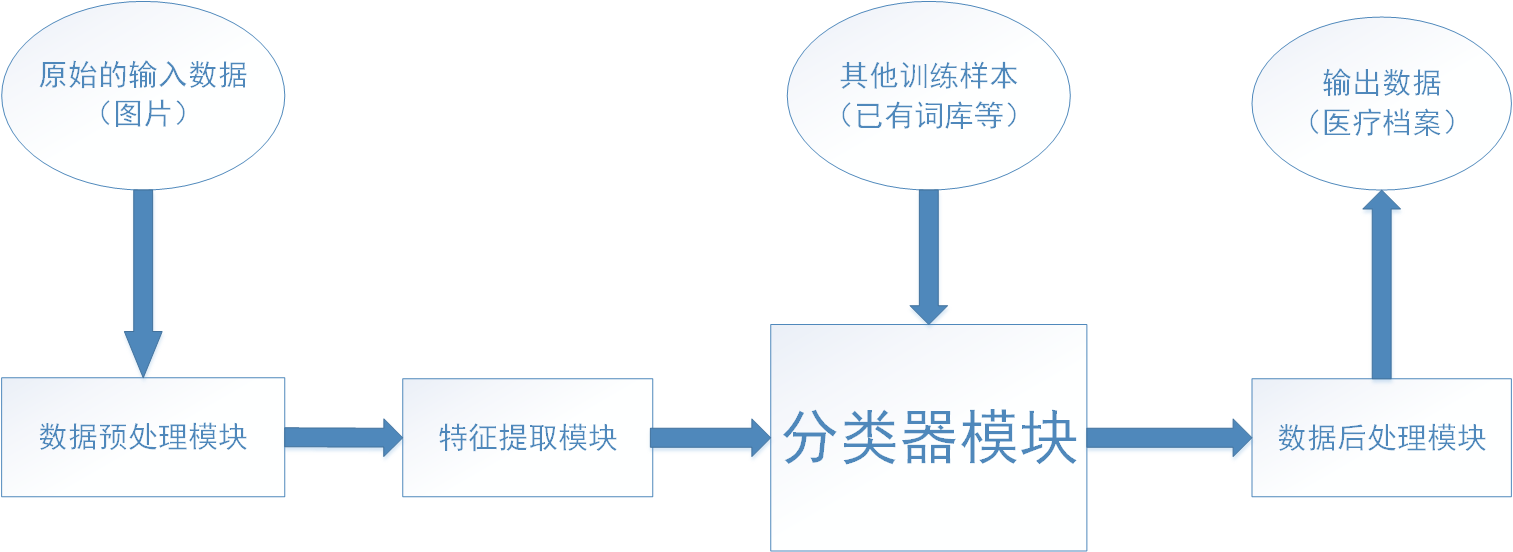
\includegraphics[scale=0.3]{figures/ocr-pipeline}
  \figcaption{光学字符识别系统的整体流程图}
  \label{pic:ocr-pipeline}
\end{figure}

\subsection{应用现状}
近几年国内对印刷体汉字识别的研究不断深入,识别准确率不断上升,也有一些较成熟的商业化产品,比较知名的有泰比(ABBYY)、中文紫光OCR、CAJViewer、清华OCR、尚书七号等。其中尤以泰比的OCR效果为佳,不仅产品线丰富、支持语言多、识别精度高,且对一些表格、框图等复杂数据有比较好的分析能力。但是,购买泰比的OCR服务是昂贵的,仅个人用户使用的专业版就售价1500元之巨,遑论针对企业用户的价格了。除了价格因素外,将现有的商业OCR系统应用到病历数据录入时,一个更棘手的问题是如果做好版面分析(Document Layout Analysis),因为病人病历数据,往往条目众多,结构复杂,不同医院病历数据的格式标准各不相同,如果直接套用商用OCR软件,识别效果是很不理想的,或者说如果没有针对病历数据的做适当的处理和调整,这些OCR软件是完全不可用的。

如何解决这个问题呢?针对病历数据格式复杂的问题,我们可以有针对性的在ocr系统中前置一个版面分析模块,将结构复杂的图片转换成简单的、便于进行文字识别的图片,再交给后续的ocr系统,将能有效的提高可用性;而针对商用OCR软件比较昂贵的问题,我们可以根据OCR系统的工作原理,自主实现一个OCR系统,即训练一个针对图片数据的文本分类器,或是采用已有的免费开源的OCR引擎,其中最为著名且效果得到广泛验证的,就是Tesseract OCR引擎。

\subsubsection{Tesseract}
Tesseract OCR引擎是一款能运行在多系统全平台(Windows,Linux,Mac,IOS,Android)的免费开源OCR引擎,最早由惠普公司Hewlett Packard实验室的工程师在1985年到1994年间开发和维护,并于2005年开放源代码,2006年之后由谷歌公司接手开发和维护\citep{wiki:Tesseract}。

在1995年,Tesseract在识别准确率上是排名前三的OCR引擎,最早的版本只支持英文,之后逐步添加多语言的支持,其中就包括中文。准确性较高、支持多语言加之免费开源,使得Tesseract在这些年,广受赞誉,是公认最好的开源OCR引擎,感兴趣的读者可访问\href{https://github.com/tesseract-ocr/tesseract}{Tesseract的GitHub主页}来获取最新的源代码。

\subsubsection{其他相关工作}
在研究领域,也有一些基于光学字符识别的应用\citep{SongWan, HongfengLi, TikunHu},这些应用也是将名片识别、车牌识别、档案识别等问题转化为光学字符识别问题,然后或自行实现简单的OCR分类器,或采用开源OCR引擎,来搭建系统,这些工作中,针对医学档案的并不多\citep{MinghuaXiang},且准确率也得不到保障,从整体完成度来看,其学术探索意味大于实际使用。

\section{本文主要工作}
本工作旨在开发一个基于中文字符识别的医学档案生成与自动归类系统,具体来说,通过针对指定病历结构的版面分析,得到结构简单明确的包含文字的图片,再加上数据预处理、开源OCR引擎Tesseract的引入和优化、病历数据矫正分类归档等,最终实现了比较精确的医学档案生成和自动归档,识别率能达到90\%以上,有较高的实用价值。同时,文章从系统的架构设计到方案选取,再到具体实现,都有着比较详尽的阐述,这对类似的应用研究与开发提供了一个参考。

\section{论文组织}
本论文的组织方式如下:
\begin{itemize}
	\item[\autoref{chap:introduction}]
	绪论,简要阐述领域背景和研究意义,分析了应用现状与相关工作,并阐明本文的主要工作。
	\item[\autoref{chap:requirements-analysis}] 需求分析,详细介绍了医学病历档案录入的实际需求和输入输出格式,分析了可能的技术难点。
	\item[\autoref{chap:system-framework}]
	架构设计,从需求出发,针对问题难点设计合理的总体框架。
	\item[\autoref{chap:implements}]
	实现细节,详细阐述了系统的核心技术和实现细节。
	\item[\autoref{chap:experiments}]
	实验,从准确率和速度维度对系统进行性能测试,并通过对比实验展示优化效果。
	\item[\autoref{chap:conclusion}]
	总结,概括性的总结本文主要工作和贡献。后续工作,分析了当前系统的不足之处,以及在后续的工作中如何解决它们。
\end{itemize}
 %第一章,绪论   3000
  \chapter{需求分析}
\label{chap:requirements-analysis}
在上一章绪论中,我们已经提到目前有大量的病历数据并没有电子化,或无法与现有的电子病历系统兼容协同,我们称之为未归档数据。从形成原因来说,未归档数据大致可以分为两大类:
\begin{itemize}
	\item 病历电子化之前的纸质档案,即现在很多医院的病历系统已经电子化,但是电子化之前的病历档案数据,仍然是纸质化的,这部分档案数据量庞大,包含了病人的历史诊疗记录,在临床上有很高的参考利用价值,故不能轻易舍弃,另一方面,旧的病历数据又很难与已有的电子化病历数据很好的协同使用,两者在档案产生、存储管理、信息展示、诊疗协助等各方面都有明显不同,为医院的诊疗工作进行提供了一些客观上的不便。
	\item 旧电子化系统中的档案,即一些医院存在着将旧的电子化病历系统废弃,采用新的电子化病历系统的情况,旧系统虽然废弃了,但是其保存的病人诊疗数据却是要保留和利用的。旧电子病历系统数据与纸质数据类似,也存在着与新电子化病历系统的协同问题,因此,如何将数据从旧系统向新系统迁移也是一个摆在面前的现实问题。
\end{itemize}
我们可以设想两个模拟的场景:
\begin{itemize}
	\item[场景A] 当一个病人去医院看病时,医生一边询问病人的主诉和症状,一边让助手去档案库中去找这个病人的过往诊疗记录,一边还要看医院电子档案系统的有关该病人的记录,纸质档案的寻找和放回都耗时耗力,面对等候在门外的患者长龙,医生可能只好根据已有的病人电子档案进行迅速诊断,这样势必会影响病人病情的综合判断。
	\item[场景B] 同样是一个病人来医院看病,医生询问病人的主诉和症状,一边的助手则根据已经录入到电子档案系统中的病人过往诊疗记录,适当提取相关信息,医生据此做出综合判断,迅速的确定病人的病情,给出来合理的治疗方案,整个过程高效且病情诊断可靠性高,病人有望迅速康复。
\end{itemize}
对比而言,场景A无疑是效率低下的,更严重是有可能影响病人病情的正确诊断,场景B则是医院的理想诊断过程,不仅效率高,且诊断更加全面准确。因此,如何将纸质病历数据和旧电子病历系统的数据迁移到新的电子化的病历系统中,是存在着广泛需求的,如果能够较好的解决这个问题,将能有效的改善现有医院病历系统的混乱现状,补全病人的医疗信息,提高诊疗效率,能给医院带来实际的效益。

\section{具体应用}
上一段中我们从总体上分析了病历档案生成与分类在医学领域的迫切需求和研究意义,现在我们更加细致的考虑这个问题,从系统角度来看,需求分析可以分别从系统环境、输入数据、输出数据以及性能这四个方面来论述。

\subsection{系统环境}
总体上,我们需要设计和实现一个病历档案生成和分类系统,系统在什么环境下运行呢?从成本、性能和稳定性等方面来综合考虑,这个系统的运行环境应该满足以下要求:
\begin{itemize}
	\item 系统能运行在普通的个人电脑上。这主要是出于成本的考虑,首先,个人电脑现在相当普及,易于获得,但是普遍性能较弱,稳定性没有保障。所以,系统应该能正常运行在性能较弱的个人电脑上。
	\item 系统能运行在商用服务器上。这主要是出于性能和稳定性上的考虑,服务器相对于个人电脑,性能更加强劲,同时,服务器有着高度的稳定性,整个系统可以很好的在服务器上长期稳定运行,持续产出,同时,服务器的一些特性也比较方便运维人员的维护和管理。
	\item 系统能对多种平台进行支持。医院内部采用的电子化系统可能运行在不同的平台上,对于主流平台,即Windows和Linux,以及Windows Server和Linux Server,系统都应该能够支持。同时,对于这些平台的不同版本(例如Windows 7和Windows XP),也要有较好的支持。
\end{itemize}

\subsection{输入数据}
\subsubsection{数据转换}
在这一章的开头,我们提到,待归档的数据主要有两类,纸质病历数据和旧电子化档案。在实际应用中,这两种数据都是不能直接被计算机系统识别的,因此,我们分别对其进行一定的转化:
\begin{itemize}
	\item 对于纸质数据,通过一台扫描仪或者照相机对病历进行录入,转换成图片数据。
	\item 对于旧电子化档案数据,我们可以在个人电脑上通过批处理的方式,打开旧电子病历,并利用个人电脑的截图功能,将病历转换成图片数据。
\end{itemize}
经过这样的转换后,这两种数据都已经转换成了图片数据,
 %第二章,需求分析  3000
  \chapter{架构设计}
\label{chap:system-framework}
当系统需求和输入输出明确以后,首先要做的就是系统的架构设计,一个好的架构设计能让系统层次简明,易于理解,各构件各司其职,从而有效提高系统的效率、稳定性、安全性、扩展性和可维护性。

\section{框架设计}
从之前的需求分析来看,医学档案自动生成与归档系统从输入图片数据,到最终输出的文档数据,需经过若干个数据处理加工步骤,这些步骤之间是顺序依次执行的,并且模块之间没有向前的反馈关系,即模块间以线性展开,没有环路,这天然构成了系统架构设计中的管道模式(Pipeline Pattern)\citep{Vermeulen1995pipeline},或称过滤器模式(Filter Pattern)。管道/过滤器模式的软件架构,是系统架构中的一种非常常见的形式,系统中每个模块都有输入输出,数据以流的形式向下传递。
它具有结构简明、扩展性好、易于维护、支持并行执行等很多优点。
具体到本系统来说,基于管道式的架构设计思想,我们可以将整个系统分成若干个处理模块,一组数据流将这些处理模块串联起来,数据流以每个病人的病历数据为单位,从输入口经过一系列加工处理,得到最终的输出,各个病人病历之间互不干扰,犹如生产线一般严格产出。

确定了采用管道式的系统架构后,接下来我们可以结合问题需求,按照数据流的顺序,一步步设计管道中的构件(模块),首先,我们需将输入的图片数据作为数据流的开端,让我们乘着数据的一叶扁舟,顺流而下,逐一分析与设计。

\section{模块设计}
\subsection{数据加载模块} \label{ssec:dataLoader-design}
数据加载模块是数据流的入口,病人病历数据以多张图片的形式输入,对于计算机而言,是无法判断某张图片是属于哪个病人的,如果不对这些图片数据进行标识,很容易出现张冠李戴的现象,现实中如果将病人A的诊疗数据误录入到病人B的病历档案中,一方面病人A的诊疗数据就此丢失,医生做诊断的时候就没法做到全面,另一方面,更严重的是医生对病人B的诊断依据的是完全错的历史诊疗记录,很可能对病人B做出不恰当的诊断,这种误诊造成的伤害是不可估量的。因此,系统对输入数据应提出这样的需求,即每个病人的病历数据应该具有唯一的标识,如图片名字拥有唯一的前缀等。而数据加载模块,就可以根据这样的标识,来给海量的图片数据做好分门别类的工作,确保数据以病人为原子单位向后传递。

\subsection{版面分析模块} \label{ssec:framework-segmentation-analysis}
当数据到达版面分析模块时,数据流中流淌的仍然是图片数据,这些图片数据中的每个“原子数据“是以病人为单位构成的一组图片集合,假设每个病人的病历数据对应着10张图片,这些图片间的病历信息互不重叠,是病历数据的有序记录,那么一个现实的问题是,当一组图片数据到来时,系统如何判断它们之间的次序,或者说某张图片中期望获得的字段数据有哪些呢?这就要求版面分析具有的第一个功能就是分辨这一组10张图片的总体属性,如果说数据加载模块是将图片数据以病人为单位做了第一步的划分,那么版面分析模块就是在此之上以图片为单位做的第二层划分。

版面分析模块的使命不止于此,当划分好每张图片后,图片中仍然存有着大量的冗余干扰信息,如\autoref{pic:input-image-1}中所示,图中除了需要识别的主题内容外,还存在着系统信息、侧边栏列表等无关信息,版面分析模块需要剔除这些干扰信息,分离出病历主题内容。

最后,对于提取出的病历主体内容,其实仍然存在着大片的空白,如果直接将它传递给下游的文字识别模块,文字相对于图片过于稀疏,识别准确率肯定大打折扣,而且识别出来的文字包含有多个字段,要从这些文字中正确解析各个字段,难度也不小。因此,版面分析模块还需要从主体内容中剔除空白内容,将各个字段提取出来,形成若干个子图片,这些子图片只包含文字区域,一个子图片对应一个字段,这样,技能有效提高后续文字识别模块的准确率,又能降低字段解析的难度,可谓一举两得。

从上面的分析来看,版面分析模块应该具备以下功能:
\begin{itemize}
	\item 对病历图片进行二次分类;
	\item 剔除图片中的干扰信息,获得病历数据主体;
	\item 剔除主体内容中的空白,提取出各个字段。
\end{itemize}
不难发现,版面分析模块本身,也可以认为是一个管道模式架构设计。

\subsection{预处理模块}
提取出来的字段图片,虽然以文字为主体,但是文字本身很可能是比较小的,从\autoref{pic:input-image-1}中就不难看出,这样的文字大小对人来说尚且有一定的辨识难度,遑论机器了,如果直接将这些图片数据丢给文字识别系统进行识别,准确性可想而知,因此,我们需要对这些文字进行必要的预处理工作,在不改变文字本身线条和结构特性的前提下,尽量放大文字尺寸和它的轮廓特征,以便文字识别模块的识别,在光学字符识别领域,预处理的好坏往往能大大影响识别精度,好的预处理能让文字识别事半功倍,反之则会成为识别精度提升的瓶颈。

\subsection{OCR模块}
接下来自然来到了整个文字识别的核心:光学字符识别(OCR)模块。光学字符识别在印刷体识别领域的应用由来已久\citep{impedovo1991optical},技术也早已成熟,其本质是一个分类器,只是输入数据被限制为图片,输出数据为文本。当识别场景简单明确时,现有的OCR技术的识别精度已经高,但是当识别场景复杂,杂讯干扰较多时,识别效果会大打折扣。所以,如果要优化OCR模块的识别效果,一方面可以从优化分类器入手,如有针对性的设计数据集、增大训练样本等,另一方面,就是前置与处理模块,将识别问题简化,有关OCR的优化,在第四章中会有更加详细的论述。
数据流经过这一个模块之后,从图片转换成了文本。

\subsection{字段解析模块}
经过OCR模块的处理,图片转换成了文字,是不是意味着大功告成了呢?显然不是。首先一个问题,就是系统其实并不能从语义上理解识别出来的文字的,因此对于机器来说,这无非是从一种无法理解的数据转换成了另外一种无法理解的数据;其次,经过OCR模块识别出来的文本,带有某些冗余信息或者是错误信息,需要进行进一步的文本清洗和矫正工作。因此,我们需要加入一个字段解析模块,既负责文本的清洗矫正工作,又承担字段解析的功能。这个模块也可以成为“后处理模块”,是对识别文本的进一步优化。

\subsection{数据存储模块}
字段被解析出来后,那么应该如何存储呢?这就需要我们整个系统最后一个模块的引入:数据存储模块。在\autoref{chap:requirements-analysis}中我们提到,需求方期望的输出是有一定的数据组织形式的、有一定可读性的最终数据,数据存储模块就是承担着数据格式的组织和存储工作的,经过它的转化之后,得到最终的需求输出。

\section{小结}
至此,我们根据病历档案自动生成与分类问题的实际需求,完成了一个管道模式/过滤器模式(Pipeline Pattern/ Filter Pattern)的系统框架设计,系统整体框架如\autoref{pic:system-framework}
所示,包含六个模块,模块间由数据流完成连接。这个框架即有一定的理论支撑,又结合病历档案系统的实际,具备比较高的可行性。
\begin{figure}
	\centering
	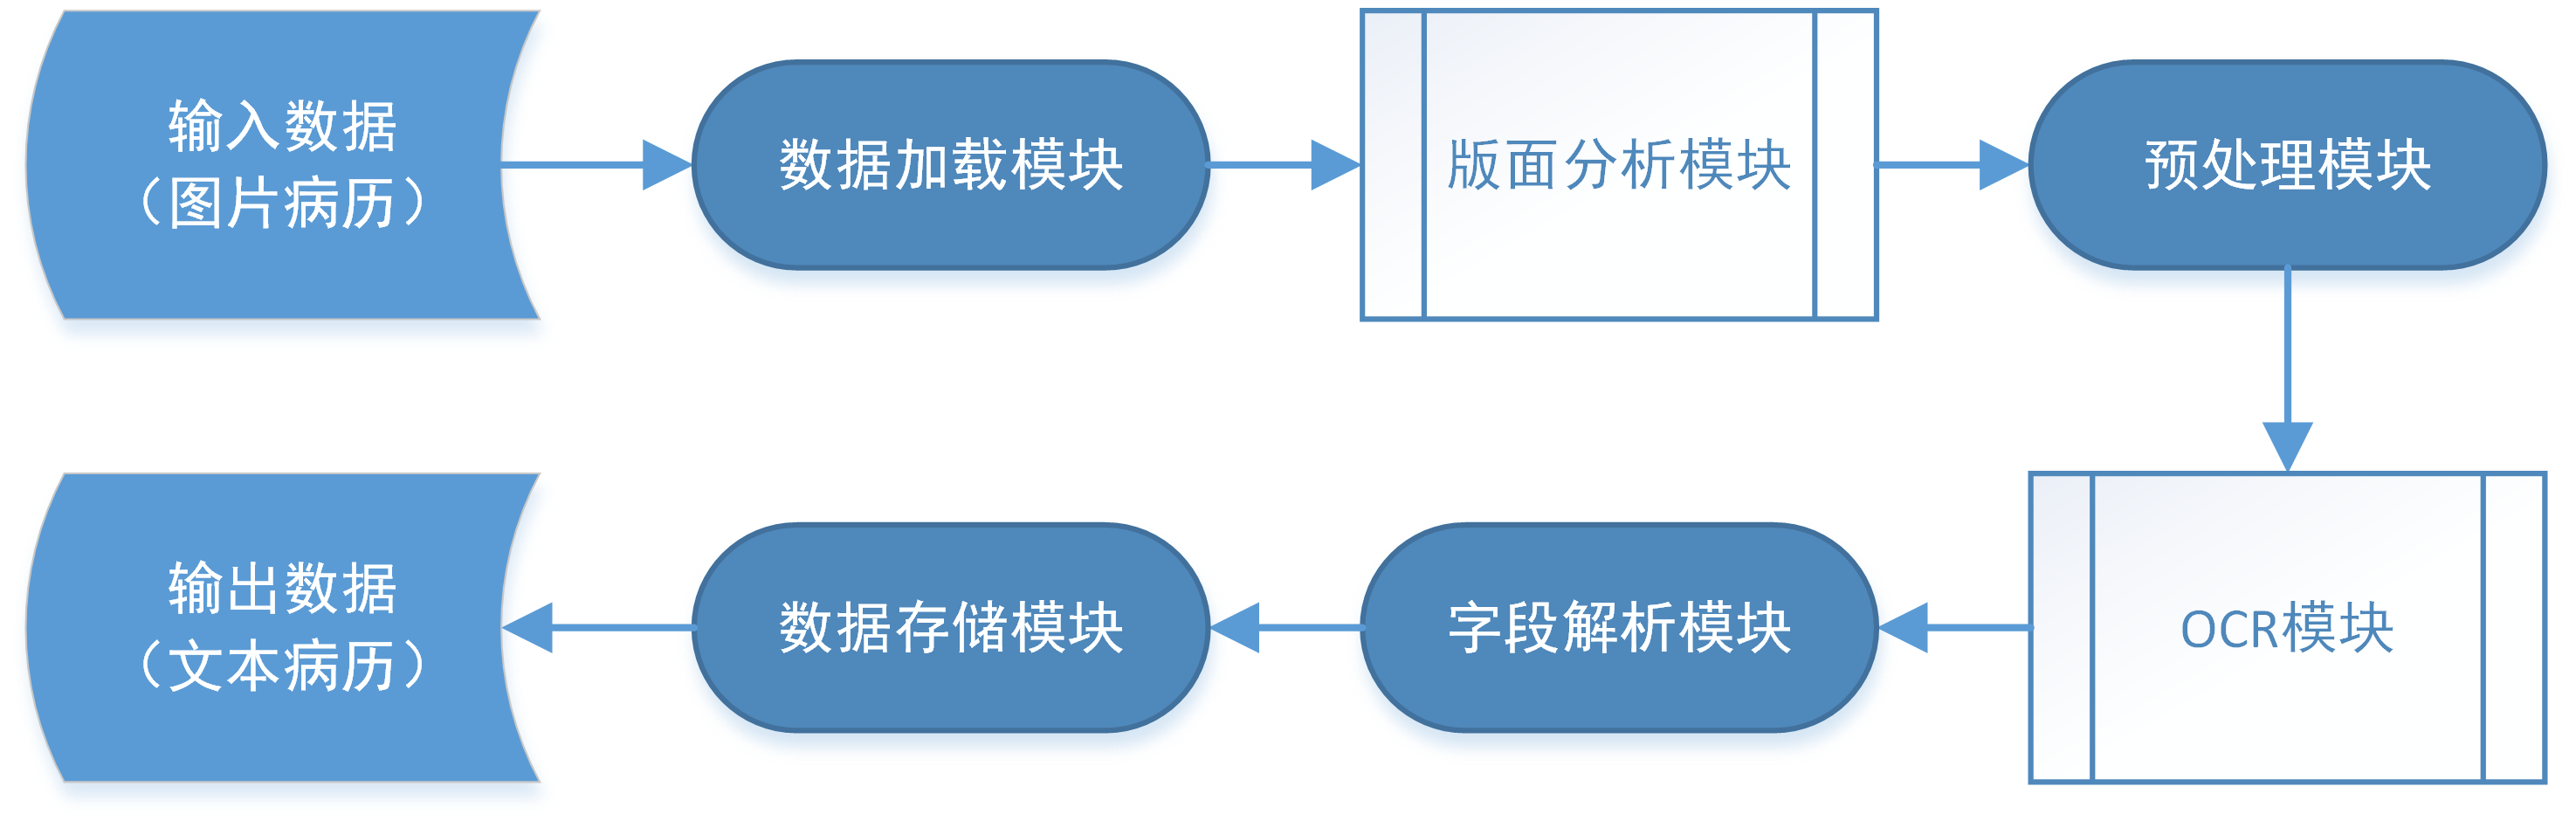
\includegraphics[width=0.9\textwidth]{system-framework}
	\caption{系统的整体架构设计}
	\label{pic:system-framework}
\end{figure}
 % 第三章,架构设计   3000
  \chapter{实现细节}
\label{chap:implements}
前一章中,我们已经介绍了整个系统的架构设计,这一章我们会对系统各个模块的一些实现细节进行详细阐述,主要涉及到方案选取、环境部署、算法设计与实现、系统性能调优等。一方面是对整体架构设计的补充论述,另一方面,我们会更多的讨论在实现过程中遇到的各种问题,以及如何解决这些问题。整体上,我们会倾向去寻找已有的成熟解决方案,辅以适当的修改和优化。遵循这个原则,既保证了整个系统有一定的成熟度,又对病历数据的识别有较强的针对性。这一部分的阐述比较详细,按照这一章的指引,有一定计算机编程基础的读者,应该能实现整个系统的基本复现。

\section{核心方案}
医学档案的自动生成与归类,其涉及到的最核心的两项技术就是图像处理和文字识别,可以说这两项技术的解决方案选取和完成度,决定了整个系统的性能基线,因此,我们必须综合考量备选的各个方案,从性能、稳定性、易用性等维度,择优采用。接下来,我们就这两项技术的方案选取和部署来展开讨论。

\subsection{图像处理}
\subsubsection{方案选取}
图像处理(Image Processing),通常又称数字图像处理,它将输入的图片、图片组或者是视频经过一系列的信号处理方面的数学转换,得到处理后的图片或是与图片相关的参数产出\citep{gonzalez2008digital}。本质来说,图像处理技术是将图片当做一个二维的信号,然后将标准的信号处理技术应用其上,当然,当图像处理技术运用到视频中时,输入变成了三维的信号,这第三维就是时间。近些年来,随着计算机视觉的蓬勃发展,图像处理技术也受到越来越多的关注。

结合前一章的分析我们可以看到,整个系统的六个模块(\autoref{pic:system-framework})中,数据加载模块、版面分析模块、预处理模块都需要用到图像处理的技术,因此我们有必要综合所有模块的需求,选取一个合适的图像处理解决方案。目前比较主流的图像处理类库有OpenCV\citep{bradski2008OpenCV}、EmguCV\citep{Shi013emgu}、AForge.net\citep{Kirillov2013Aforge}、CImg\citep{tschumperle2012cimg}等,在\citep{XianrongWang}的文章中,作者对几大主流的的图像处理库在各个维度做了一个比较全面的对比。从\autoref{pic:image-processing-comparison}中可以看到,OpenCV在性能上,是其中的佼佼者,也是最为广泛使用的图像处理类库,在功能上,也能完全满足本系统的图像处理要求,故经过比较后,系统决定采用它作为图像处理的解决方案。

\begin{figure}
	\centering
	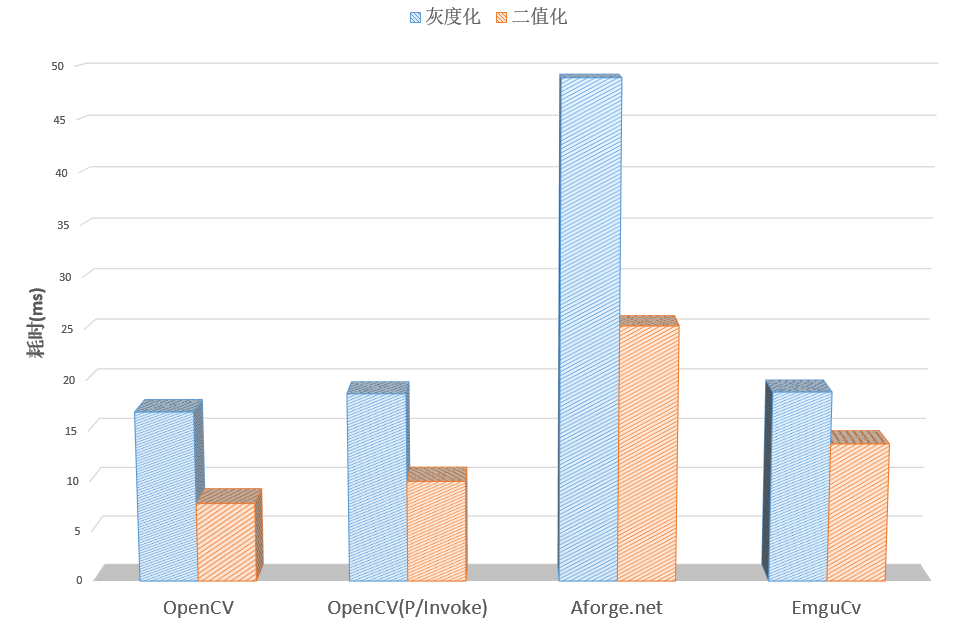
\includegraphics[width=0.9\textwidth]{Image-Processing-Comparison}
	\caption{几种图像处理库的性能比较}
	\label{pic:image-processing-comparison}
\end{figure}

OpenCV(Open Source Computer Vision)是一个旨在完成实时机器视觉(Real-time Computer Vision)的函数库,最早是由英特尔研究中心开发,后被Will Garage接手,现在是由Itseez团队负责维护,是一个跨平台的免费开源图像处理库\citep{wiki:OpenCV}。OpenCV最早于2000年发行,目前仍在更新和维护,最新的稳定版是于2015年12月发布的OpenCV 3.1更新。它的代码由C/C++写就,同时提供了Python、Java以及Matlab等语言的接口\citep{wiki:OpenCV}。自其发布后的15年来,OpenCV一直以它良好的性能和高度的稳定性著称,是使用最为广泛的图像处理库。这也意味着它有着大量的用户测试经验和成熟的社区支持,这无疑为我们解决项目中的棘手问题提供了基础保障,具体来说,本系统的数据加载模块、版面分析模块、预处理模块都需要用到OpenCV提供的函数方法支持,我们也将在后面的模块详细介绍中,体会到OpenCV的强大功能。

\subsubsection{环境部署}
OpenCV是有很好的多平台支持(Windows,Linux,Mac等),环境的部署也比较简单,这里我们仅以Windows平台下Visual Studio 2013的opencv配置使用为例,做一个部署步骤的简要展示:
\begin{itemize}
  \item 从\href{http://opencv.org/}{OpenCV官方主页}下载最新的OpenCV 3.1安装包,解压安装包完成安装。并将OpenCV加入系统环境变量。
  \item 新建一个Visual Studio C++工程,在工程配置属性中的“包含目录”中添加OpenCV的include文件夹,在“库目录”中加入OpenCV的lib文件夹,在“链接器”的附加依赖中添加opencvworld310d.lib和opencvworld310.lib(分别对应debug和release编译选项)。
  \item 在工程中添加如下测试代码OpenCV-test.cpp(代码见下方,功能是展示示例图片),编译运行,如果编译通过,并且程序正确开辟“example”窗口并显示示例图片,说明OpenCV的环境就配置成功了。
\end{itemize}

\begin{Codex}[label=OpenCV-test.cpp, numbers=left]
#include <iostream>
#include "opencv2/highgui/highgui.hpp"
using namespace cv;
int main(void)
{
  Mat img = imread("example.jpg", 0);
  imshow("example", img);
  waitKey();
  return 0;
}
\end{Codex}

上面只是简述了OpenCV的部署步骤,具体到不同的平台和软件版本,部署时会有一些小的差异,读者可结合自己的情况,从网络上找到对应的详细部署指南,这里就不再赘述了。

\subsection{字符识别}
\subsubsection{方案选取}
字符识别(Character Recognition),又称光学字符识别(Optical Character Recognition,OCR),是指将印刷或手写的文字转换成机器编码(machine-encoded)文本的过程,它被广泛应用于纸质印刷的数据录入中,例如护照文件、发票、信件、银行存单等,当这些纸质文件被转换成了机器编码的文本以后,无论是在编辑修改、搜索、存储,还是在后续的数据挖掘,文字转语音等过程中,都变得相对便捷和高效。OCR是模式识别(Pattern Recognition)、(Artificial Intelligence)和计算机视觉(Computer Vision)领域中的典型应用\citep{wiki:OCR}。

具体到本系统,我们是要讲光学字符识别技术应用到纸质或截图保存的病历数据中,这项技术会在OCR模块中用到,在技术实现上与其他基于光学字符识别的应用并没有本质的不同,因此我们可以采用已有的OCR解决方案。目前比较主流的OCR解决方案有ABBYY FineReader、Microsoft Office内置的OCR模块、Tesseract、FreeOCR等,维基百科中有对各种OCR软件的详细对比\citep{wiki:OCRcomparison},同时,也有组织对于最好的OCR软件做过一个排名(见\autoref{pic:ocr-software-comparison}),从这个排名中我们可以看到,好的商用OCR软件一般都售价不菲(图片中的价格仅针对个人用户),同时由于病历数据的版面结构复杂,并没有一个比较通用的版面分析方案,所以这些商用OCR软件无法直接应用到系统中,因此,我们需要一个有提供编程接口(Application Programming Interface,API)的OCR解决方案,方便定制特定场景下的OCR。能提供编程接口的OCR引擎中,Tesseract是其中的首选。

\begin{figure}
	\centering
	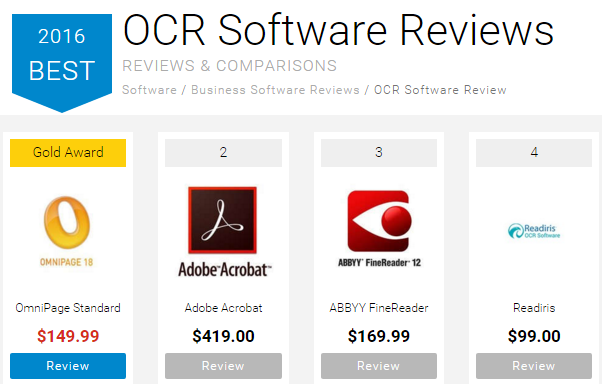
\includegraphics[width=0.9\textwidth]{ocr-software-comparison}
	\caption{某组织对现有OCR软件的排名}
	\label{pic:ocr-software-comparison}
\end{figure}

Tesseract OCR引擎是一款能运行在多系统全平台(Windows,Linux,Mac,IOS,Android)的免费开源OCR引擎,最早由惠普公司Hewlett Packard实验室的工程师在1985年到1994年间开发和维护,并于2005年开放源代码,2006年之后由谷歌公司接手开发和维护\citep{wiki:Tesseract}。

在1995年,Tesseract在识别准确率上是排名前三的OCR引擎,最早的版本只支持英文,之后逐步添加多语言的支持,其中就包括中文。准确性较高、支持多语言加之免费开源,使得Tesseract在这些年,广受赞誉,是公认最好的开源OCR引擎,读者可访问\href{https://github.com/tesseract-ocr/tesseract}{Tesseract的GitHub主页}来获取最新的源代码。同时,Tesseract的源码是由C/C++编写,与同样是C/C++编写的OpenCV图像处理库能够很好的兼容,事实上,Tesseract也开发了专门针对OpenCV的API接口,提供了丰富的支持。综上,系统决定采用Tesseract作为字符识别的解决方案。

\subsubsection{环境部署}
Tesseract支持多平台(Windows,Linux,Mac)使用和开发,如果只是简单使用tesseract,可以下载安装包安装Tesseract的可执行程序,如果需要基于Tesseract进行二次开发,则需要编译它的源代码,显然,我们的需求属于后者。接下来本文以Windows平台下Visual Studio 2013的Tesseract编译为例,做一个简要的环境部署展示:
\begin{itemize}
	\item 安装版本控制软件Git\footnote{更多相关信息可访问Git官方网站:https://git-scm.com/}。
	\item 在电脑中建立tesseract-build文件夹,在该文件夹下打开CMD控制台程序,并分别运行:
	\begin{Code}[numbers=left]
git clone git://github.com/charlesw/tesseract-vs2012.git
git clone git://github.com/tesseract-ocr/tesseract.git
	\end{Code}
	\item 打开VS 2013 Developer Command Prompt,然后输入命令:
	\begin{Code}[numbers=left]
msbuild "${tesseract-build}\tesseract-vs2012\build.proj"
	\end{Code}
	其中\$\{tesseract-build\}表示tesseract-build这个文件夹在电脑中的绝对路径。
	\item 将vs2013+64bit\_support.batch文件拷贝到tesseract-build文件夹下,然后进入到tesseract文件夹,执行以下命令:
	\begin{Code}[numbers=left]
git checkout -b 3.04-vs2013 3.04.00
git am --signoff ../vs2013+64bit_support.patch
	\end{Code}
	\item 将tesseract-build$\backslash$tesseract-vs2012$\backslash$release目录下的所有文件拷贝到tesseract-build目录下。
	\item 用VS2013打开tesseract-build$\backslash$tesseract$\backslash$vs2013下的tesseract.sln工程,开始编译,如果编译正常通过,就说明环境已经配置完成。
\end{itemize}

上面的只是一个配置过程的简述,不同平台、不同版本之间的配置方式有着比较明显的差异,需结合自身的情况,选取对应的配置部署流程,这里不再详述。

\section{数据加载模块}  %500字

1.可添加简单的容错处理
2.忽略已经写入过的文件夹

\section{版面分析模块}  % 3000字
文档版面分析(Document Layout Analysis),是指在含有文本的图像中识别出感兴趣区域(Regions of Interest,ROI)的过程。一个文字识别系统需要将文字从非文字的区域中划分出来,同时保持文本的相对顺序\citep{baird1992anatomy}。在一个文件中检测和标记出文本区域和其他非文本区域的过程叫做几何学版面分析(Geometric Layout Analysis)\citep{cattoni1998geometric}。但是不同的文本区域在文档中代表的含义并不相同,例如有些文本是文档的标题,有些是文档的注释,有些是文档的主体等等,具体到病历档案归类系统中,就是文本块所属的字段是各不相同的,这种识别文字在文档中的含义的过程叫做逻辑学版面分析(Logical Layout Analysis)\citep{haralick1994document}。

(几何学)版面分析算法总体上可以分为三类\citep{mao2003document}:
\begin{itemize}
	\item 自顶向下方法,算法从整张图片开始,迭代地将图片不断分割成更小的区域,直到程序达到某种终止条件时停止。它的优点是操作简单、速度较快,但是难以适应比较复杂的版面\citep{nagy1992prototype}\citep{baird1990image}。
	\item 自底向上方法,与自顶向下的方法相反,算法从每一个图片像素开始,根据一定的聚即规则,逐渐聚集相邻的区域形成单词,语句和段落。它的优点是能够适应比较复杂的版面,缺点是速度比较慢,难以确定一个比较好的聚集规则\citep{o1993document}\citep{kise1998segmentation}。
	\item 混合型方法,它可以被看做是自顶向下和自底向上这两种方法的混合\citep{pavlidis1992page}。
\end{itemize}

在真实的应用场景中,由于实际文档的多样性,复杂性,因此,目前还没有一个固定的,最优的切割模型,需要我们根据实际问题和需求,有针对性的设计版面分析方法。在\autoref{ssec:framework-segmentation-analysis}中我们已经提到,系统的版面分析模块非常重要,需要完成以下三大功能:
\begin{itemize}
	\item 对病历图片进行二次分类;
	\item 剔除图片中的干扰信息,获得病历数据主体;
	\item 剔除主体内容中的空白,提取出各个字段。
\end{itemize}
这三个功能我们可以简单归纳为图片分类、主体保留、字段提取。这三者的顺序是从逻辑上出发来区分的,在实际代码实现中,我们是先实现了主体保留,此时再对图片分类,最后做字段提取的工作。接下来,我们分别讨论这三个功能如何实现。

\subsection{主体保留}
图片中除了我们需要的病历主体信息以外,一般还会有冗余的干扰信息,以\autoref{pic:input-image-1}为例,图片的中间部分是病人病历数据的主体,而图片上部则是一些电子病历系统的系统信息,左侧则是一个侧边栏导航,这些都是与病历无关的,我们需要将其剔除,保留主体,这里需要用到图片的裁剪。

\subsubsection*{OpenCV中矩形框裁剪}
在OpenCV中,可以很方便的根据矩形框来裁剪,假如原始图片已转换为Mat格式\footnote{Mat是OpenCV 2.x中图片加载以后的格式},名字为origin,我们需要产生的裁剪图片为cut,那么裁剪的代码为:
\begin{Code}
cut = origin( Rect(x0, y0, width, height) );
\end{Code}
其中$(x_0,y_0)$表示裁剪区域的左上角在原图中的位置,width和height则分别表示裁剪区域的宽度和高度。

现在我们知道用OpenCV裁剪矩形图片了,但是对于\autoref{pic:input-image-1}这样的数据,我们怎么确定$(x_0,y_0)$和width、height呢?

\subsubsection*{模板匹配}
需要注意的是,在确定的病历系统中,其系统信息和侧边栏导航的内容和位置是相对固定的,我们可以根据这一点,利用模板匹配的方式,确定系统信息栏和侧边导航栏的位置,并进行裁剪。

模板匹配(Template Matching)\citep{template-matching},是一项在原始图片中寻找匹配模板图片的小区域的技术。在OpenCV中,提供了模板匹配的函数
\begin{Code}
void matchTemplate(InputArray image, InputArray templ, OutputArray result, int method)
\end{Code}
其中image表示原始图像,templ表示模板图像,result为结果矩阵,method为匹配算子类型。具体匹配过程为模板图像在原始图像中滑动,根据不同的匹配算子,计算重叠区域的匹配度,当滑动过整个原始图像区域后,返回匹配度最高的子图像信息。

OpenCV提供了6种默认的匹配算子,最常见的是平方差匹配算子(\autoref{eq:square})和相关匹配算子(\autoref{eq:correlation}):
\begin{equation} \label{eq:square}
R(x,y)=\sum_{x^{'},y^{'}}(T(x^{'},y^{'})-I(x+x^{'},y+y^{'}))^2
\end{equation}

\begin{equation} \label{eq:correlation}
R(x,y)=\sum_{x^{'},y^{'}}(T(x^{'},y^{'})\cdot I(x+x^{'},y+y^{'}))
\end{equation}
其中,$T(x^{'},y^{'})$表示模板图像中的点,$I(x+x^{'},y+y^{'})$表示原始图像滑动窗口中对应的点。平方差匹配算子衡量的是两者的差别,所以这个值越低,说明匹配度越高,而相关匹配算子衡量的是两者的相关性,所以这个值越高,说明匹配度越高。

\begin{figure}
	\centering
	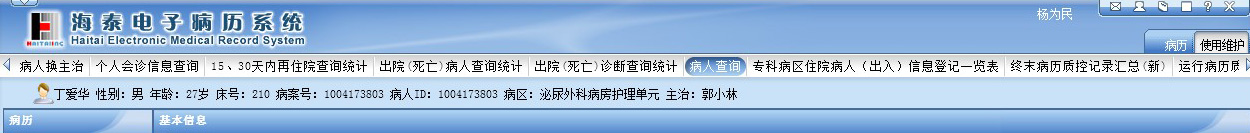
\includegraphics[width=0.9\textwidth]{title-template}
	\caption{系统信息栏模板}
	\label{pic:title-template}
\end{figure}

对于病历图片中的系统信息栏,我们可以通过截取原图中系统信息栏的部分保存下来,作为模板,如\autoref{pic:title-template}所示。然后运用模板匹配算法,剪裁掉原图中上方系统信息栏部分,代码如下:(其中算子采用平方差算子,输入参数src代表原图,\_template代表模板,template\_type为模板类型,返回值roi为截掉模板之后的图像。)
\begin{Codex}[label=Cut,numbers=left]
Mat MatchingMethod(Mat src, Mat _template, int template_type)
{
	// template_type option:  0 -> title, 1 -> sidebar
	Mat result;
	int match_method = CV_TM_SQDIFF_NORMED;
	Mat img_display;
	src.copyTo(img_display);
	int result_cols = src.cols - _template.cols + 1;
	int result_rows = src.rows - _template.rows + 1;
	result.create(result_rows, result_cols, CV_32FC1);
	matchTemplate(src, _template, result, match_method);
	normalize(result, result, 0, 1, NORM_MINMAX, -1, Mat());
	double minVal; double maxVal; Point minLoc; Point maxLoc;
	Point matchLoc;
	minMaxLoc(result, &minVal, &maxVal, &minLoc, &maxLoc, Mat());
	matchLoc = minLoc;
	Mat roi;
	if (template_type)
	roi = src(Rect(matchLoc.x + _template.cols, matchLoc.y, src.cols - matchLoc.x - _template.cols, _template.rows));
	else
	roi = src(Rect(0, matchLoc.y + _template.rows, matchLoc.x + _template.cols, src.rows - matchLoc.y - _template.rows));
	return roi;
}
\end{Codex}

去掉系统信息栏之后的图像如\autoref{pic:template-cut-title}所示,接着我们采用同样的方法,也可去掉侧边的导航栏,最终得到\autoref{pic:template-cut-title}所示,可以看到,病历的主体已经被完整的剥离出来,至此,主体保留的工作就完成了。

\begin{figure}[htbp]
  \centering
  \subfloat[]{
  \label{pic:template-cut-origin}
  \begin{minipage}[t]{0.3\textwidth}
    \centering
    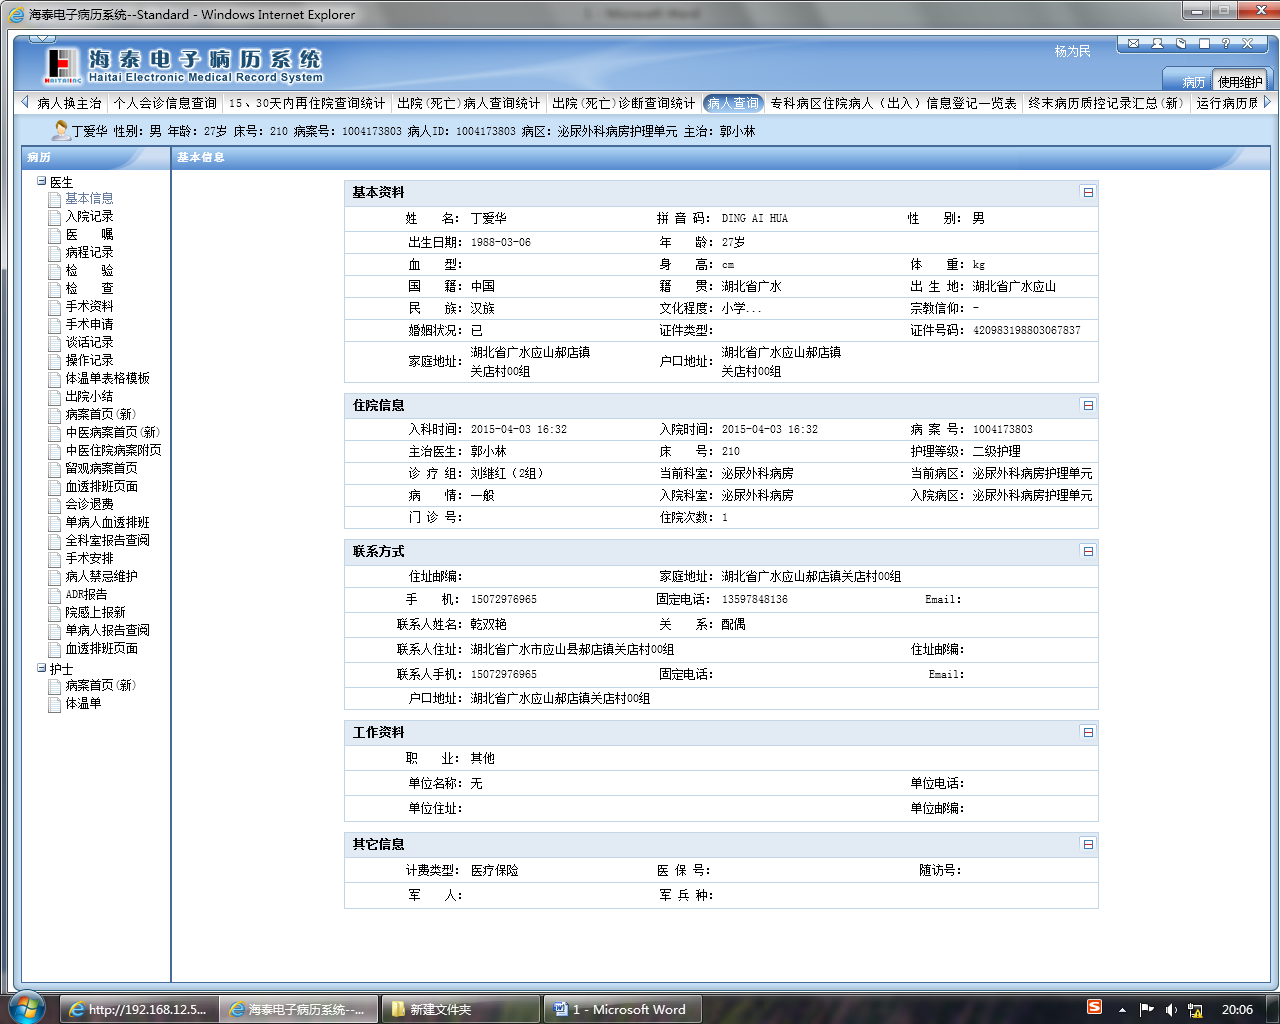
\includegraphics[width=\textwidth]{input-image-1}
  \end{minipage}
  }
  \subfloat[]{
  \label{pic:template-cut-title}
  \begin{minipage}[t]{0.3\textwidth}
    \centering
    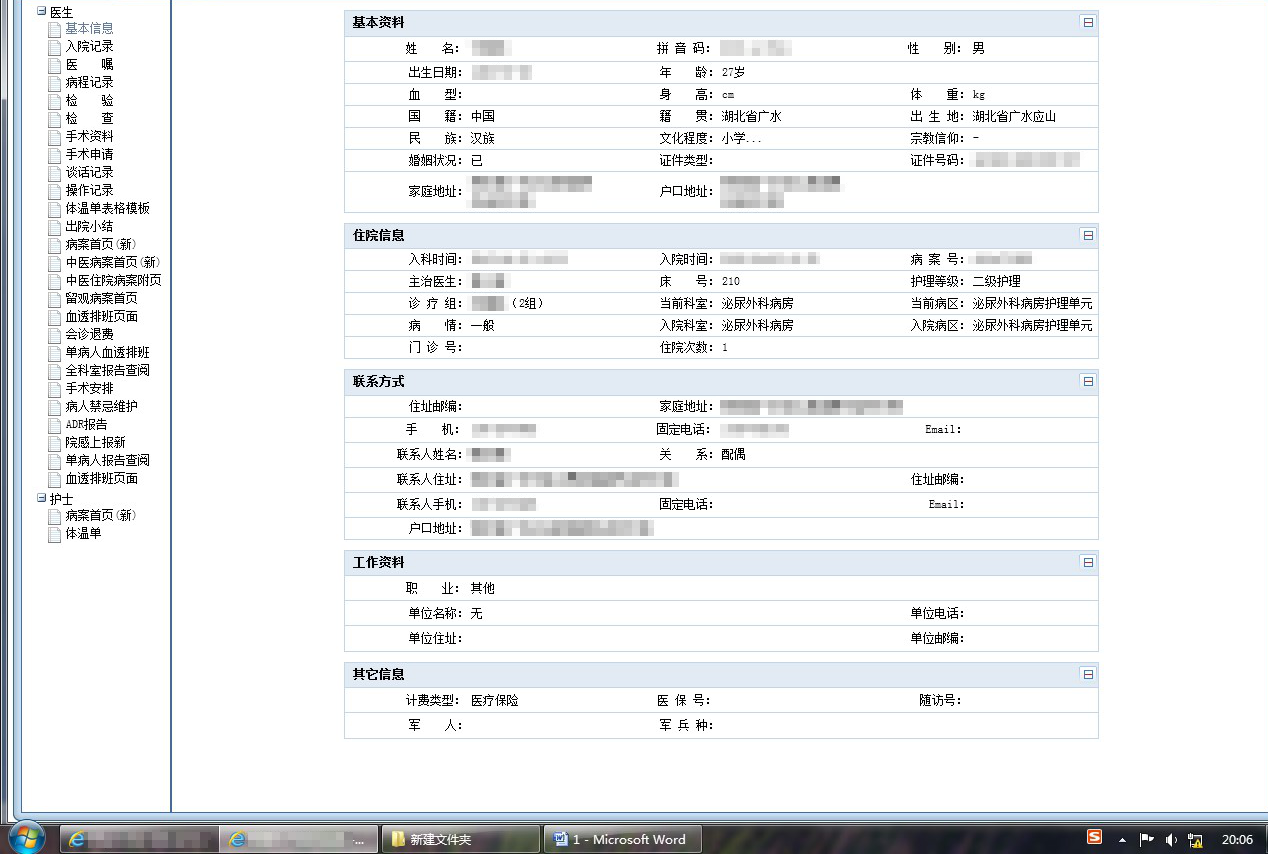
\includegraphics[width=\textwidth]{cut_title}
  \end{minipage}
  }
  \subfloat[]{
  \label{pic:template-cut-sidebar}
  \begin{minipage}[t]{0.3\textwidth}
    \centering
    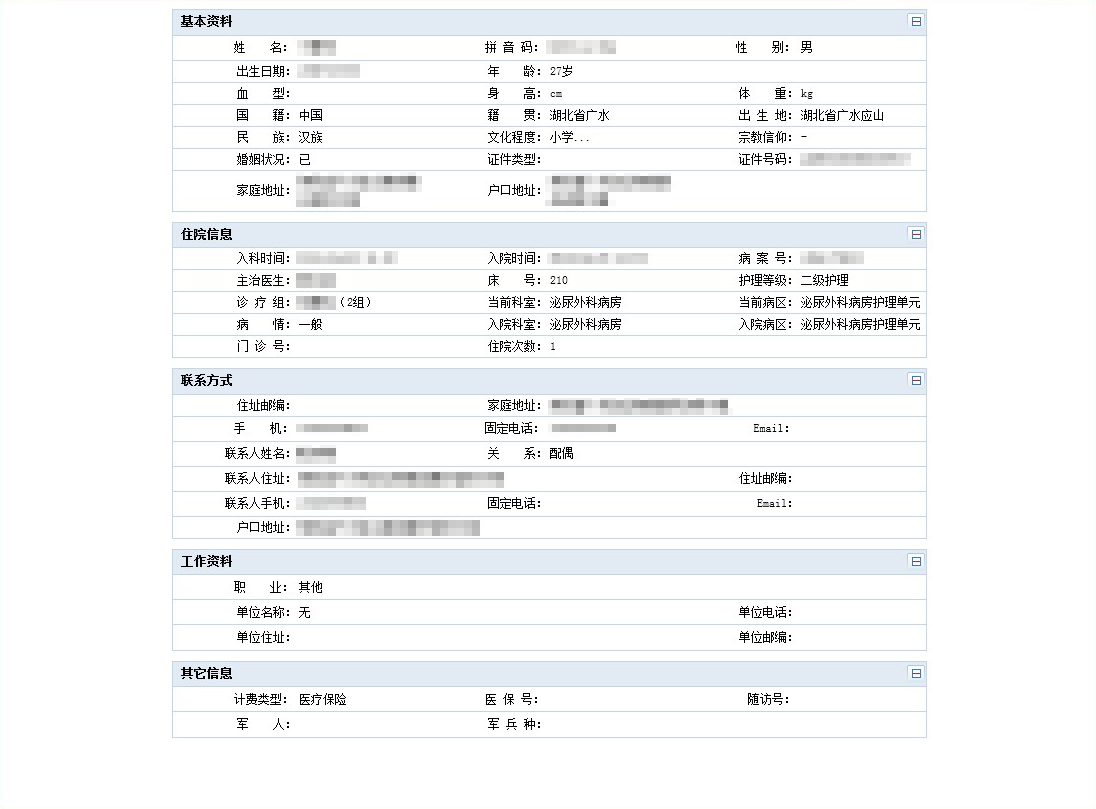
\includegraphics[width=\textwidth]{cut_sidebar}
  \end{minipage}
  }
  \caption{病历主体内容截取}
  \label{pic:different-layout}
\end{figure}

\subsection{图片分类}
在\autoref{ssec:framework-segmentation-analysis}中,我们已经提到每个病人对应着大约7到10张图片,这些图片的内容互不重复,加起来构成了完整的病人诊疗信息,图片之间的版式是各不相同的,如\autoref{pic:different-layout}所示,三张图片都属于同一个病人的病历数据,但是主体内容的版式各不相同,\autoref{fig:sub-input-image-1}中主要记录的是病人的基本信息,如姓名、性别等,\autoref{fig:sub-input-image-3}中记录的则是病人详细的病情数据,而\autoref{fig:sub-input-image-2}则介于两者之间。假设病人的病历图片只有这三种样式,那么当有一张图片输入时,应该如何判断这张图片属于哪个样式呢?这就涉及到图片相似度(image similarity measure)度量的问题了。

\begin{figure}[htbp]
  \centering
  \subfloat[]{
  \label{fig:sub-input-image-1}
  \begin{minipage}[t]{0.3\textwidth}
    \centering
    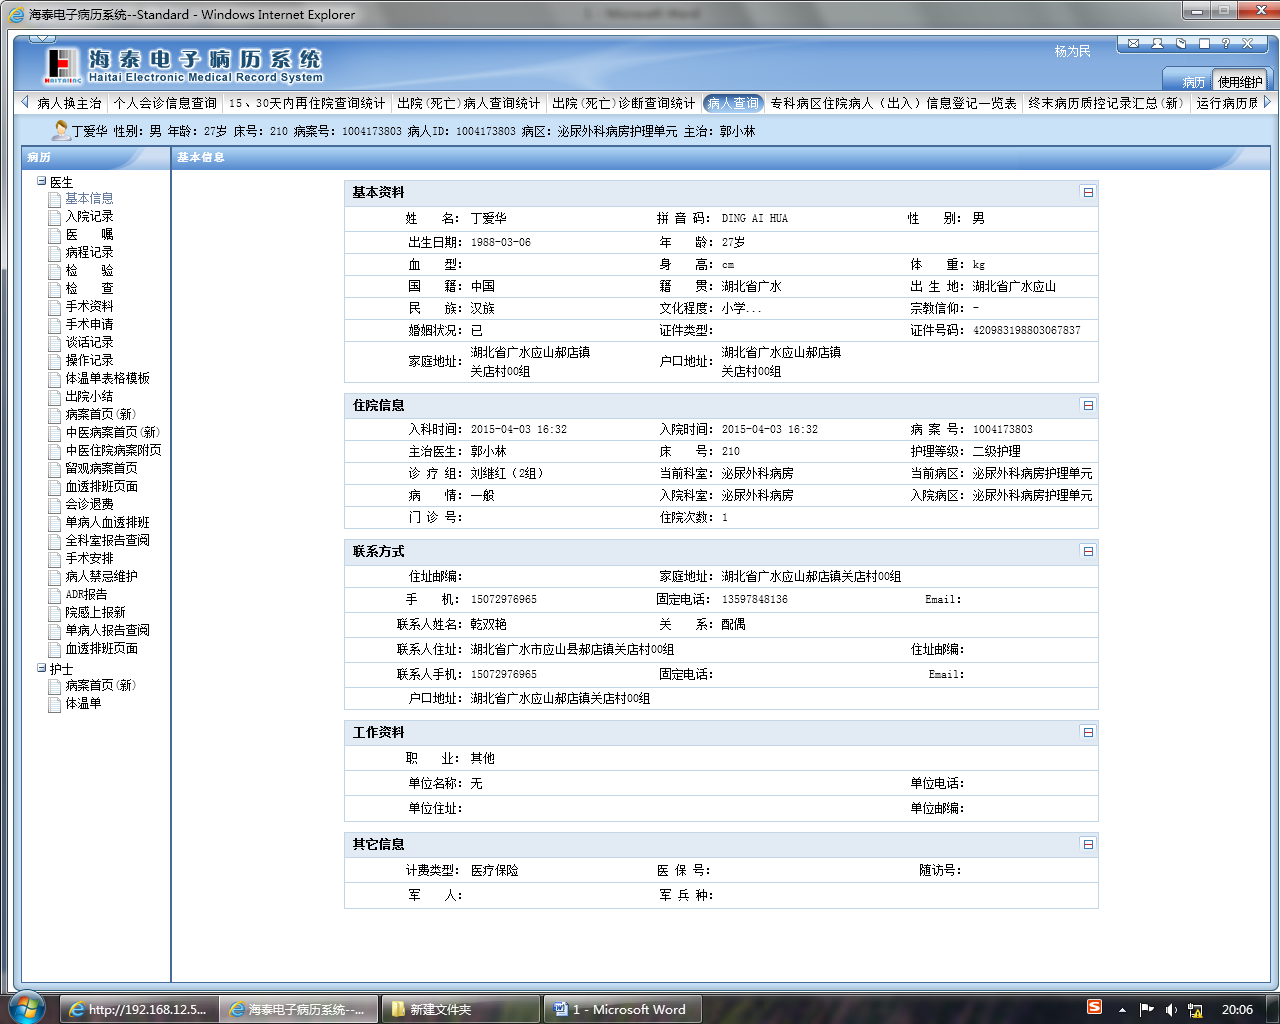
\includegraphics[width=\textwidth]{input-image-1}
  \end{minipage}
  }
  \subfloat[]{
  \label{fig:sub-input-image-2}
  \begin{minipage}[t]{0.3\textwidth}
    \centering
    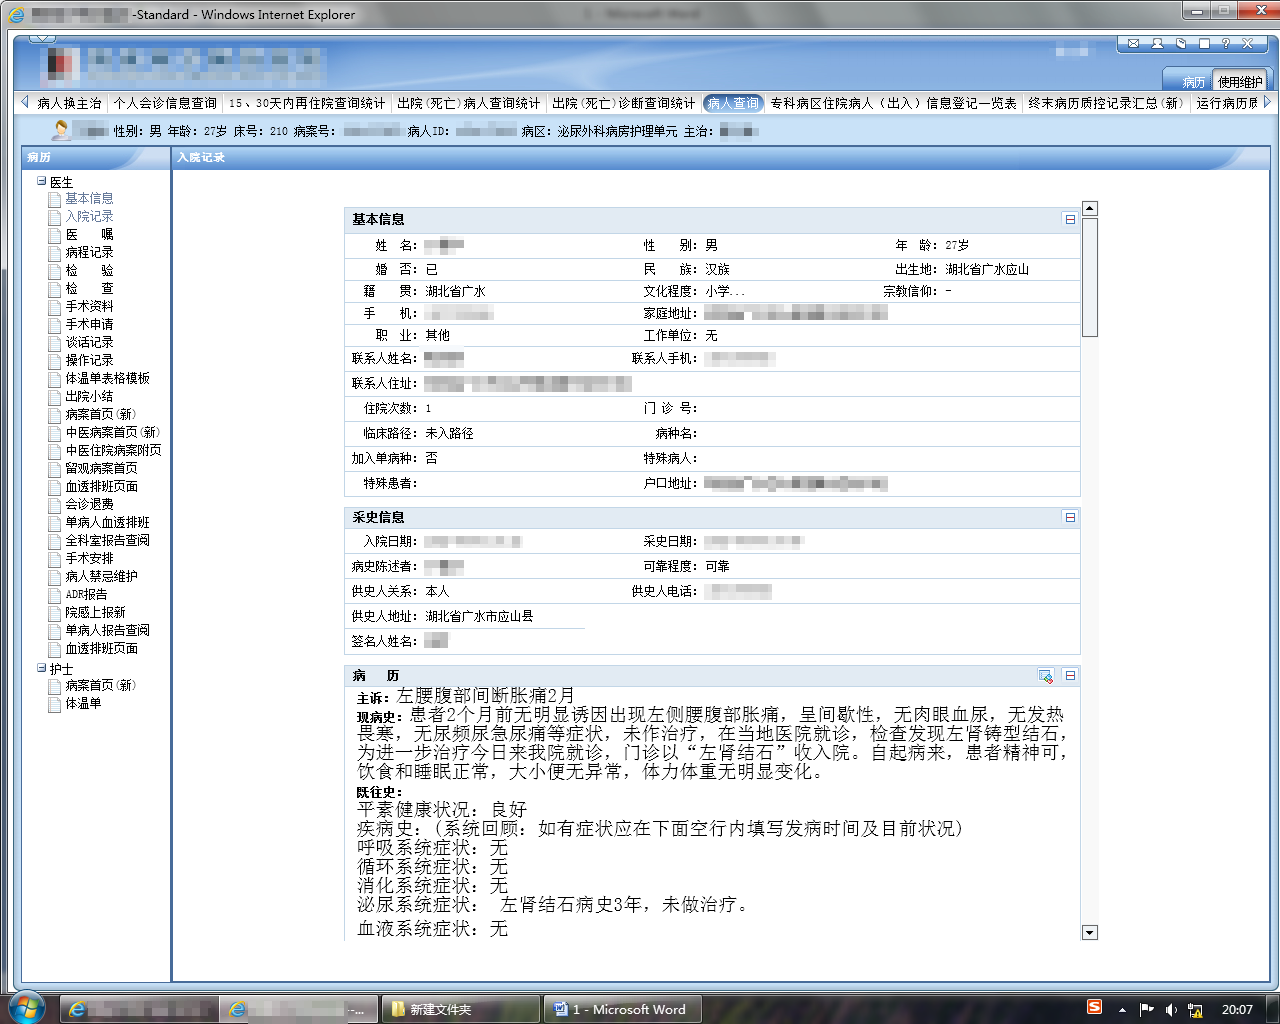
\includegraphics[width=\textwidth]{input-image-2}
  \end{minipage}
  }
  \subfloat[]{
  \label{fig:sub-input-image-3}
  \begin{minipage}[t]{0.3\textwidth}
    \centering
    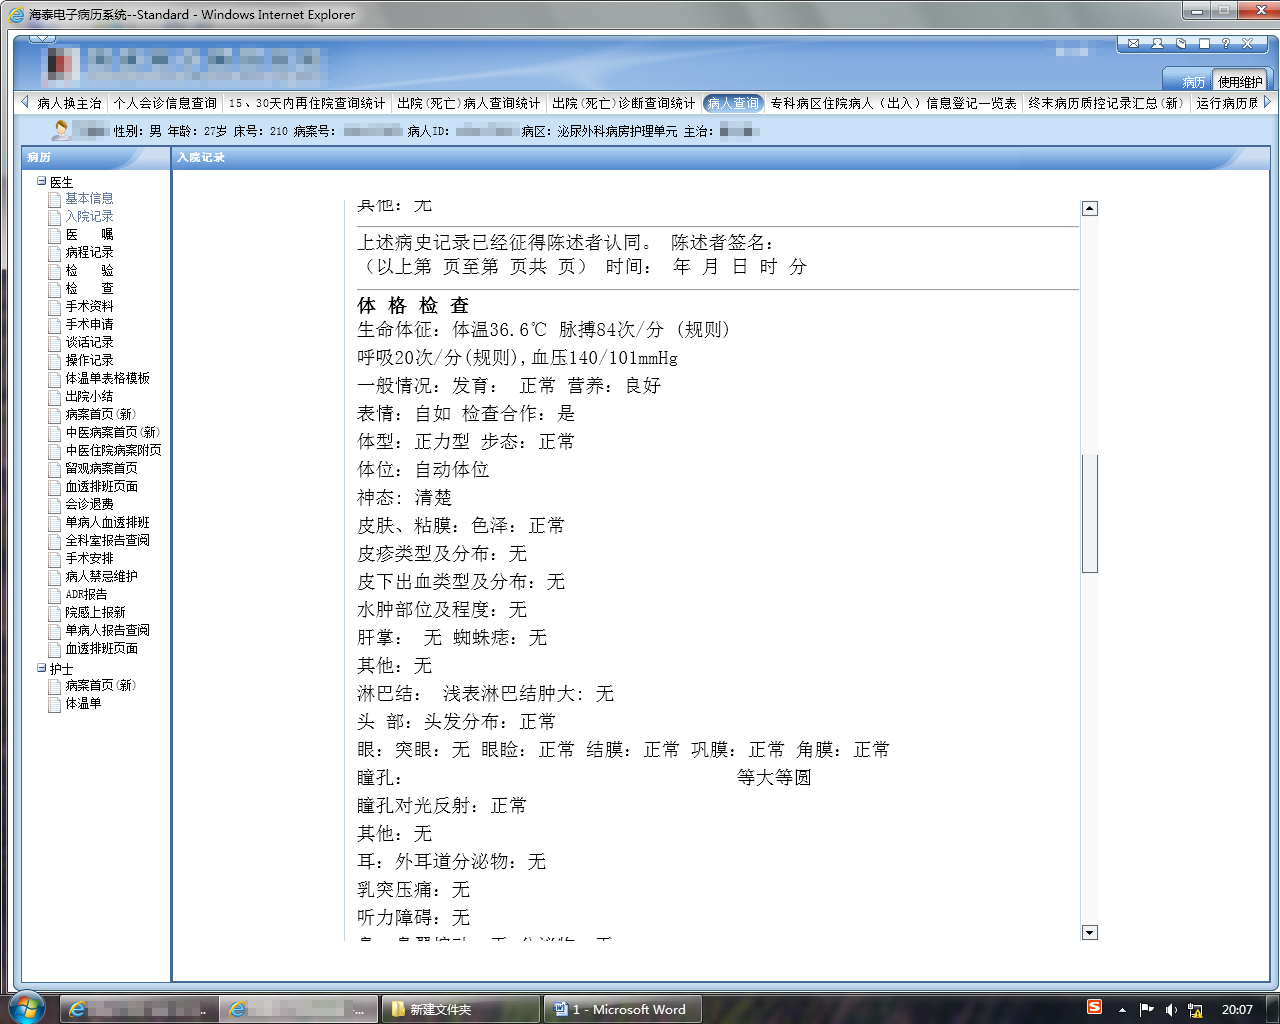
\includegraphics[width=\textwidth]{input-image-3}
  \end{minipage}
  }
  \caption{病历图片的几种版式}
  \label{pic:different-layout}
\end{figure}

相似性度量(Similarity Measure)\citep{lin1998information},或者距离度量(Distance Meature),是一个用来定义两个物体相似性或者距离的实值函数\citep{singhal2001modern},常见的相似性度量函数有欧几里得距离(Euclidean distance)\citep{wiki:Euclidean-distance}、余弦距离(Cosine Distance)\citep{wiki:Cosine-distance}、机器学习中的核函数(Kernel Functions)\citep{hofmann2008kernel}等等,这些相似性度量在数据挖掘领域有着广泛的应用\citep{tan2006introduction}。图片相似度度量,是相似性度量的一个特例,当然,版式作为图片信息的一个抽象,它的相似度度量是图片相似度度量的一个子集。一般来说,图像相似性度量分为两个部分\citep{goldberger2003efficient}:
\begin{itemize}
  \item 图像表示(Image Representation),既然相似性度量是一个实值函数,那么图片数据需要转换成某种数值的表示形式才能进行度量,比较常见的表示方法是将图片中的每个像素分成红绿蓝三个维度的0-255的整数值进行存储,而灰度、二值等都是不同的图片表示方法。
  \item 相似度定义与计算,定义一个合适的相似度度量指标,计算图片间的相似度。这个是与问题相关的,不同问题适用的相似度度量也不一样。
\end{itemize}
具体到病历图片版面相似性度量,由于我们的病历图片的版式只有固定的几种,假设为三种,这样对于每张图片,我们可以与这三种版式分别进行相似性比较,相似度最高的就是该图片的版式。但是对于同一种版式,各个字段的内容是不相同的,比如姓名字段,每个病人的名字就各不相同,因此,我们需要预先对图片做一些处理,抛弃一些细节信息,消除因为各个字段内容不同造成的整体相似度的差异。这里就需要用到图像处理中图片的灰度化、二值化、腐蚀等操作了,我们先来逐一介绍下这几种图像转换方法。

\subsubsection*{灰度化}
\label{sub:灰度化}
一张彩色图像在计算机中是由若干个像素点的形式存在,像素点的多少取决于图像的分辨率PPI(Pixel Per Inch),而每个像素点最常见的表示形式是RGB(Red,Green,Blue,即红。绿。蓝)三原色,三原色的不同组合比例能表示丰富的色彩。而灰度图(Greyscale Image)则是另外一种表示形式,它只保存了每个像素的亮度(Intensity)信息,将RGB图像转换为灰度图需满足\autoref{eq:RGBtoGray}:
\begin{equation} \label{eq:RGBtoGray}
		\begin{split}
& P(x,y) = \alpha R(x,y) + \beta G(x,y) + \gamma B(x,y),  \\
& where \quad \alpha,\beta,\gamma > 0,\alpha + \beta + \gamma = 1
		\end{split}
\end{equation}
其中,$P(x,y)$表示像素点的灰度值,$R(x,y),G(x,y),B(x,y)$表示像素点的三原色值,系数$\alpha,\beta,\gamma$的一个常见取值为$\alpha=0.299,\beta=0.587,\gamma=0.114$。从\autoref{eq:RGBtoGray}中我们可以知道,灰度转换实际上是从RGB三维到灰度一维的投影,这种转换会损失信息,并且是不可逆的。\autoref{pic:greyscale}展示了RGB图像灰度化以后的结果。

\begin{figure}[htbp]
  \centering
  \subfloat[]{
  \label{pic:lena}
  \begin{minipage}[t]{0.45\textwidth}
    \centering
    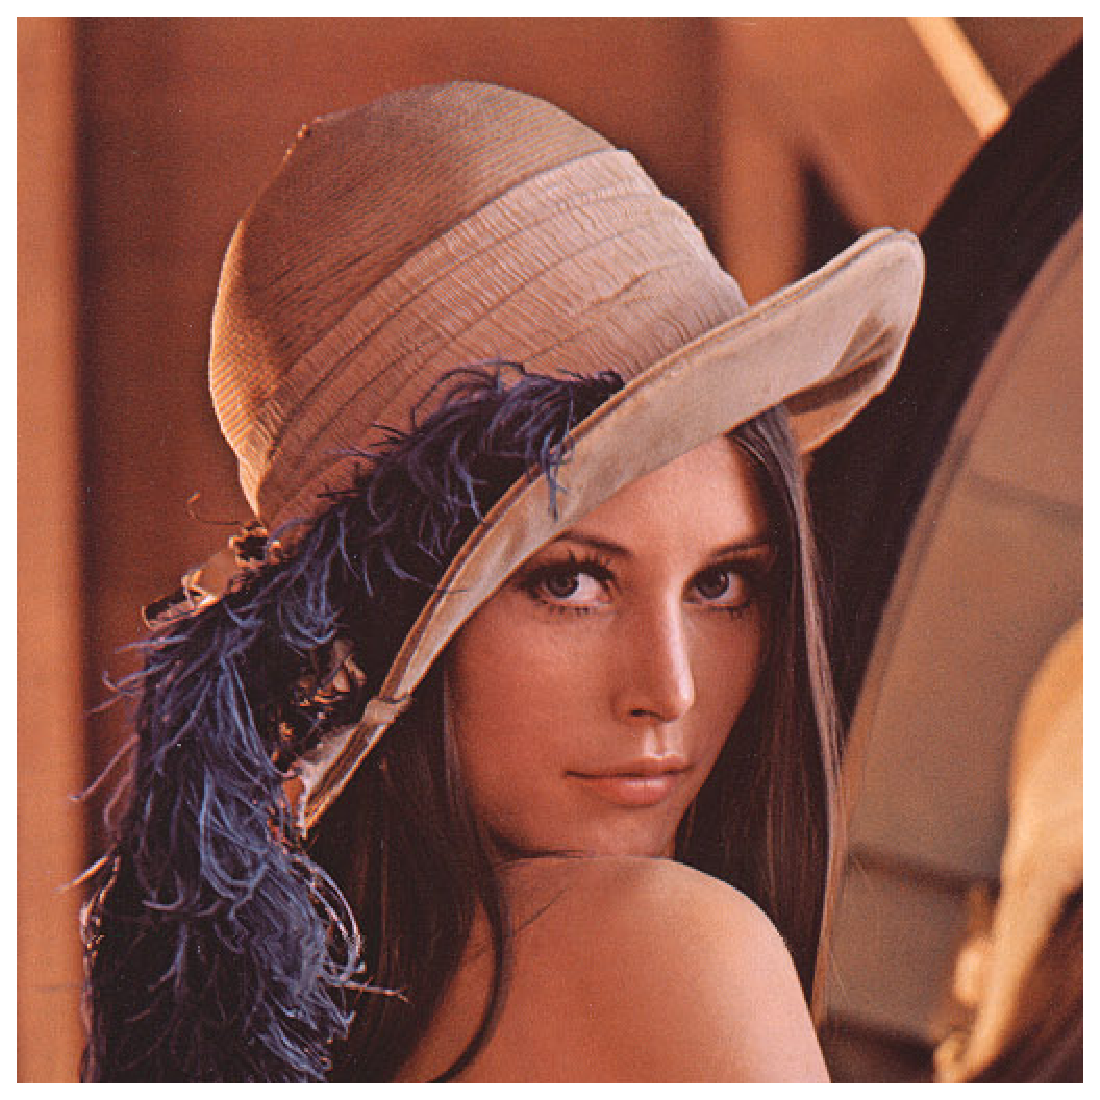
\includegraphics[width=\textwidth]{lena}
  \end{minipage}
  }
	\hfill
  \subfloat[]{
  \label{pic:lena-grey}
  \begin{minipage}[t]{0.45\textwidth}
    \centering
    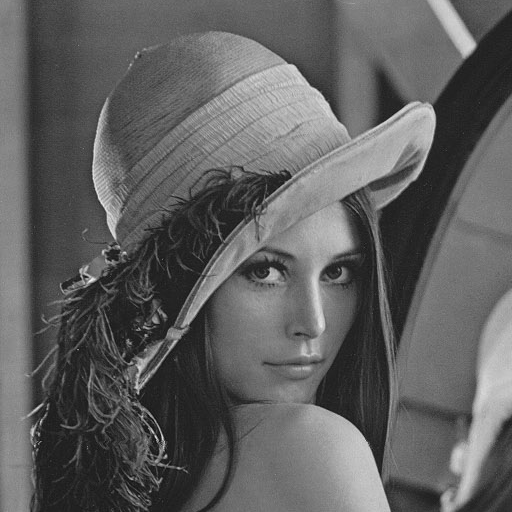
\includegraphics[width=\textwidth]{lena_grey}
  \end{minipage}
  }
  \caption{图片的灰度化}
  \label{pic:greyscale}
\end{figure}

\subsubsection*{二值化}
\label{sub:二值化}
二值化图像(Binary Image)中,每个像素只有两种可能的值,分别是黑和白,将灰度图二值化的过程满足\label{pic:binarization}:
\begin{equation} \label{pic:binarization}
	B(x)=
	\begin{cases}
		0,&x\geq threshold\cr 1,&x<threshold
	\end{cases}
\end{equation}
其中$x$表示像素点的灰度值(常见取值为$0-255$),$threshold$为二值化的阈值,当$x$大于阈值时,该像素点为白色,反之为黑色。OpenCV提供了两种二值化方法,分别是固定阈值方法和自适应阈值方法。

固定阈值方法,即需要事先指定一个全局阈值,根据这个阈值对灰度图进行二值化,函数原型为
\begin{Code}
double threshold(InputArray src, OutputArray dst, double thresh, double maxval, int type)
\end{Code}
固定阈值方法虽然实现简单,但是阈值需要人工选取,很难保证效果,当阈值选的太大时,会产生很多噪声,淹没主体(见\autoref{lena_binary_130}),阈值选的太小时,又会丢失大量的细节(见\autoref{lena_binary_70}),因此这种方法在具体实施时并不推荐。

自适应阈值方法,函数原型为
\begin{Code}
void adaptiveThreshold(InputArray src, OutputArray dst, double maxValue, int adaptiveMethod, int thresholdType, int blockSize, double C)
\end{Code}
它根据像素的邻域块的像素值分布来确定该像素位置上的二值化阈值。这样做的好处在于每个像素位置处的二值化阈值不是固定不变的,而是由其周围邻域像素的分布来决定的。亮度较高的图像区域的二值化阈值通常会较高,而亮度较低的图像区域的二值化阈值则会相适应地变小。不同亮度、对比度、纹理的局部图像区域将会拥有相对应的局部二值化阈值。常用的局部自适应阈值有:1)局部邻域块的均值;2)局部邻域块的高斯加权和。%这一段摘自http://blog.csdn.net/icvpr/article/details/8515596
自适应阈值二值化效果见\autoref{lena_binary_adaptive},图片即保证了主体的明确,没有很多噪声,又保留了大部分的细节。

\begin{figure}[htbp]
  \centering
  \subfloat[]{
  \label{pic:lena_binary_origin}
  \begin{minipage}[t]{0.45\textwidth}
    \centering
    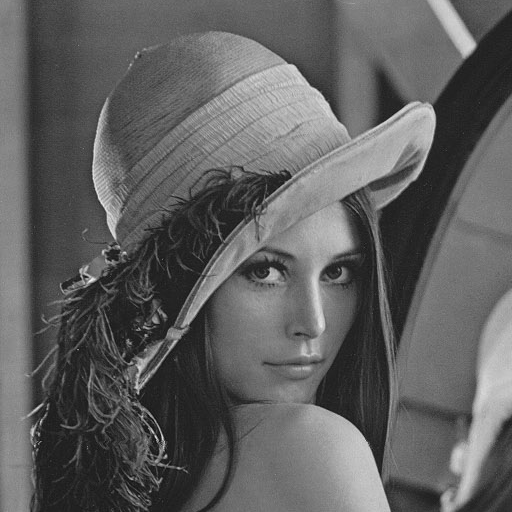
\includegraphics[width=\textwidth]{lena_grey}
  \end{minipage}
  }
	\hfill
  \subfloat[]{
  \label{pic:lena_binary_130}
  \begin{minipage}[t]{0.45\textwidth}
    \centering
    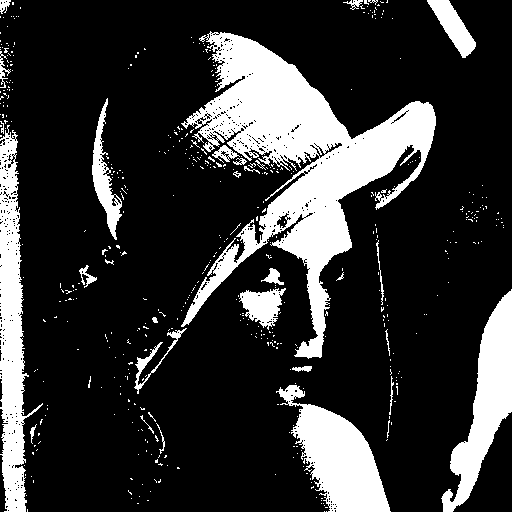
\includegraphics[width=\textwidth]{lena_binary_130}
  \end{minipage}
  }
	\vskip\baselineskip
  \subfloat[]{
  \label{pic:lena_binary_70}
  \begin{minipage}[t]{0.45\textwidth}
    \centering
    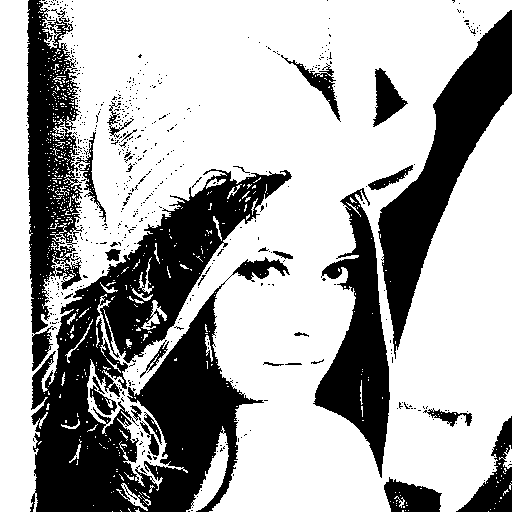
\includegraphics[width=\textwidth]{lena_binary_70}
  \end{minipage}
  }
	\hfill
  \subfloat[]{
  \label{pic:lena_binary_adaptive}
  \begin{minipage}[t]{0.45\textwidth}
    \centering
    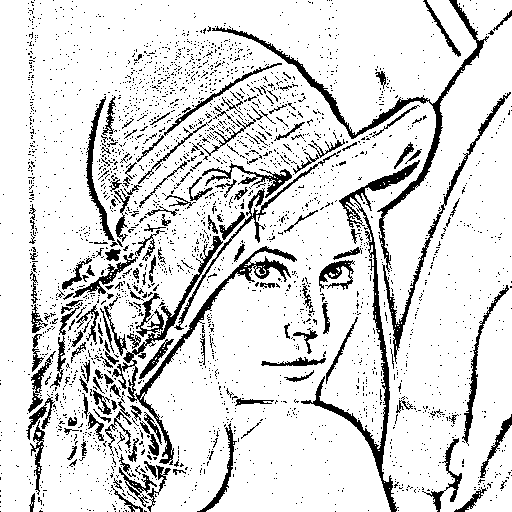
\includegraphics[width=\textwidth]{lena_binary_adaptive}
  \end{minipage}
  }
  \caption{不同二值化方法的差别}
  \label{pic:different-binary-approach}
\end{figure}

\subsubsection*{图像的膨胀和腐蚀}
图像的膨胀和腐蚀是两种常见的图像形态学操作(Morphological Operations),形态学操作简而言之,就是根据一个结构化元素(Structuring Element)对输入图片进行一系列基于外形的图像处理操作,得到输出图片。图像的膨胀和腐蚀在很多方面都有应用,例如去噪、个体元素提取或连接等。

膨胀(Dilation),可以被看做一个是基于某个核(Kernel)$B$的卷积(convoluting)操作,这个核$B$可以是任意的形状和大小,一般来说是方形或者是原型,
核$B$一般有一个预先定义好的锚点(anchor point),一般来说是核的中心。当核$B$依次扫过图片的时候,在$B$与图片的重叠区域,算法会计算区域内的最大值,并将当前锚点的值替换为这个最大值,显然,这样的最大化操作会使图片中比较亮的区域扩张,如\autoref{pic:dangan}中,\autoref{pic:dangan_origin}是包含有“档案”两个字的原图,\autoref{pic:dangan_dilated}则是经过膨胀操作以后的效果。

腐蚀(Erosion),则可以被认为是膨胀的“反操作”,即当核$B$扫过原图时,将锚点的值替换为重叠区域的最小值,这种最小化操作会使图片中比较亮的区域收缩,对应的暗色区域扩展,图片的腐蚀效果可见\autoref{pic:dangan_eroded}。

\begin{figure}[htbp]
  \centering
  \subfloat[]{
  \label{pic:dangan_origin}
  \begin{minipage}[t]{0.3\textwidth}
    \centering
    
\includegraphics[width=\textwidth]{dangan_origin}
  \end{minipage}
  }
  \subfloat[]{
  \label{pic:dangan_dilated}
  \begin{minipage}[t]{0.3\textwidth}
    \centering
    
\includegraphics[width=\textwidth]{dangan_dilated}
  \end{minipage}
  }
  \subfloat[]{
  \label{pic:dangan_eroded}
  \begin{minipage}[t]{0.3\textwidth}
    \centering
    
\includegraphics[width=\textwidth]{dangan_eroded}
  \end{minipage}
  }
  \caption{图片的膨胀和腐蚀}
  \label{pic:dangan}
\end{figure}

对图片的灰度化、二值化、膨胀和腐蚀操作有所了解以后,我们就可以利用这些图像处理方法,来进行图片分类任务了。前面我们提到我们是通过比较图片与三种版式图片的相似性来确定图片的版式,如\autoref{pic:layout-comparison}中所示,\autoref{pic:bingli1-cut}、\autoref{pic:bingli2-cut}、\autoref{pic:bingli3-cut}分别是保留主体的模板版式,而\autoref{pic:new-bingli1-cut}则是需要确定版式的新图片,我们只需要确定新图片与三张模板版式图片哪张最接近,就可以确定新图片的版式了。以我们的肉眼判断,测试图片的版式与\autoref{pic:bingli1-cut}是最接近的,但是,对于计算机来说,并不是那么容易判断。
\begin{figure}[htbp]
  \centering
  \subfloat[版式1]{
  \label{pic:bingli1-cut}
  \begin{minipage}[t]{0.23\textwidth}
    \centering
    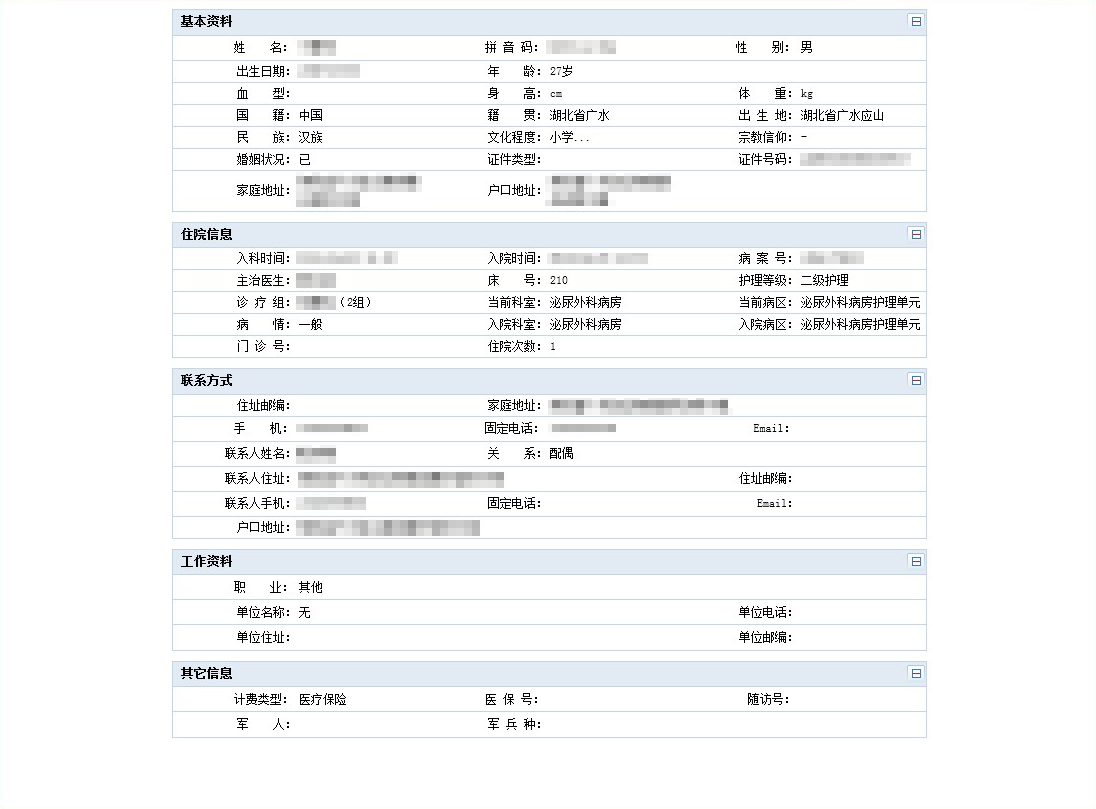
\includegraphics[width=\textwidth]{cut_sidebar}
  \end{minipage}
  }
	\hfill
  \subfloat[版式2]{
  \label{pic:bingli2-cut}
  \begin{minipage}[t]{0.23\textwidth}
    \centering
    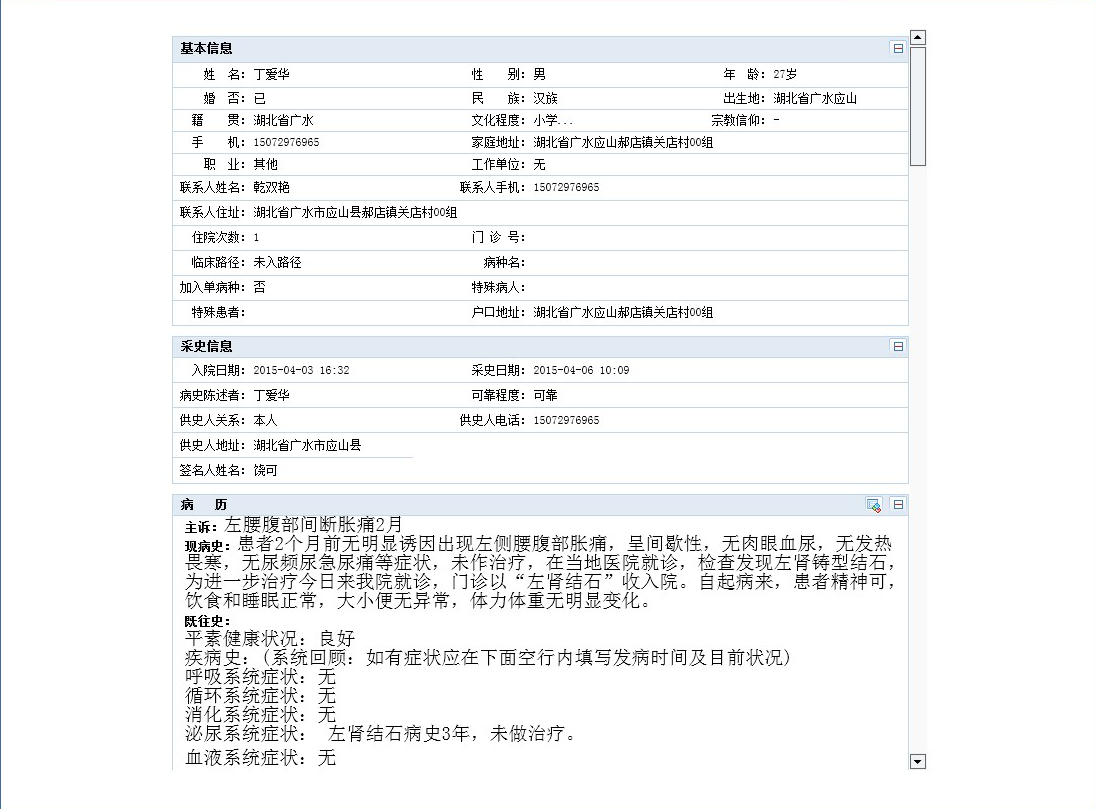
\includegraphics[width=\textwidth]{bingli2-cut}
  \end{minipage}
  }
  \subfloat[版式3]{
  \label{pic:bingli3-cut}
  \begin{minipage}[t]{0.23\textwidth}
    \centering
    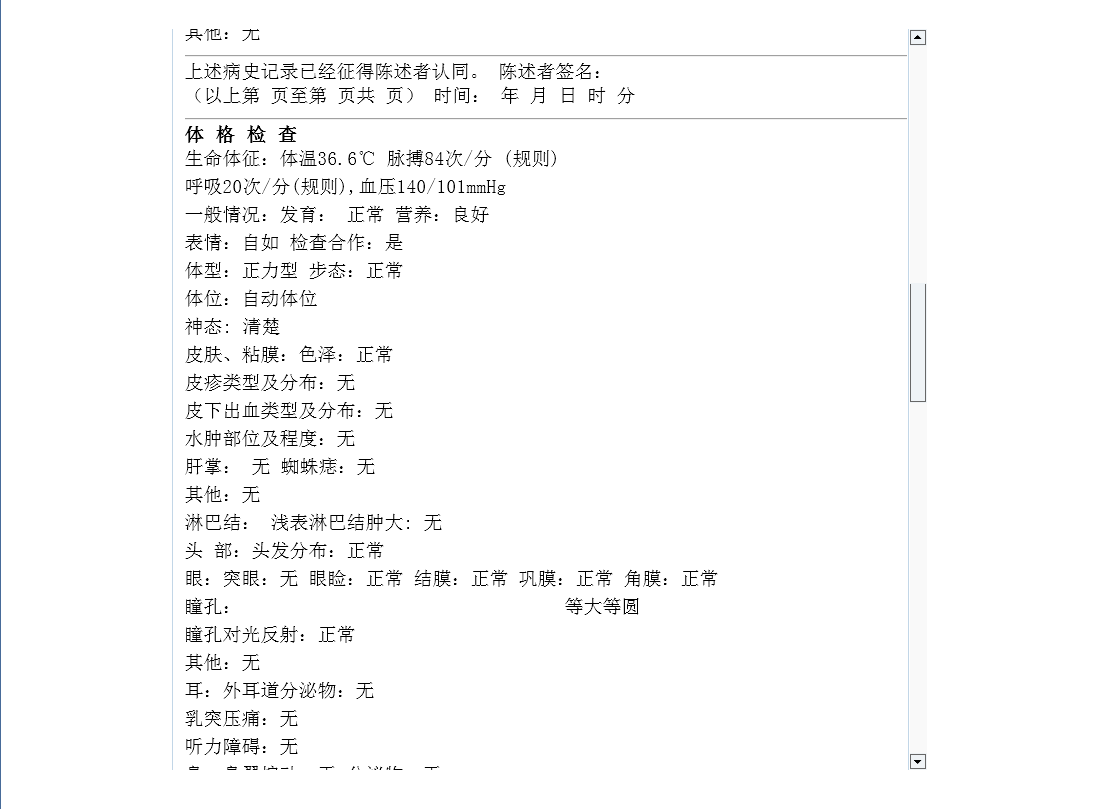
\includegraphics[width=\textwidth]{bingli3-cut}
  \end{minipage}
  }
	\hfill
  \subfloat[测试图]{
  \label{pic:new-bingli1-cut}
  \begin{minipage}[t]{0.23\textwidth}
    \centering
    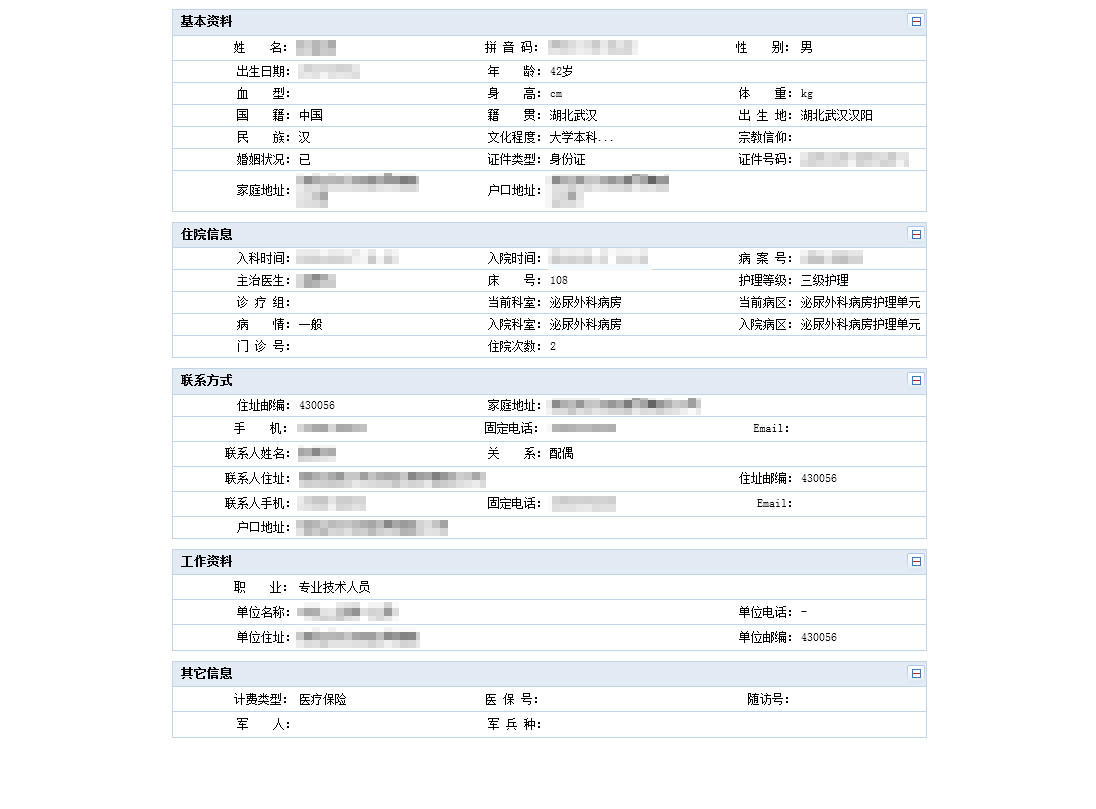
\includegraphics[width=\textwidth]{new-bingli1-cut}
  \end{minipage}
  }
	\vskip\baselineskip
  \subfloat[变换后的版式1]{
  \label{pic:bingli1-cut-eroded}
  \begin{minipage}[t]{0.23\textwidth}
    \centering
    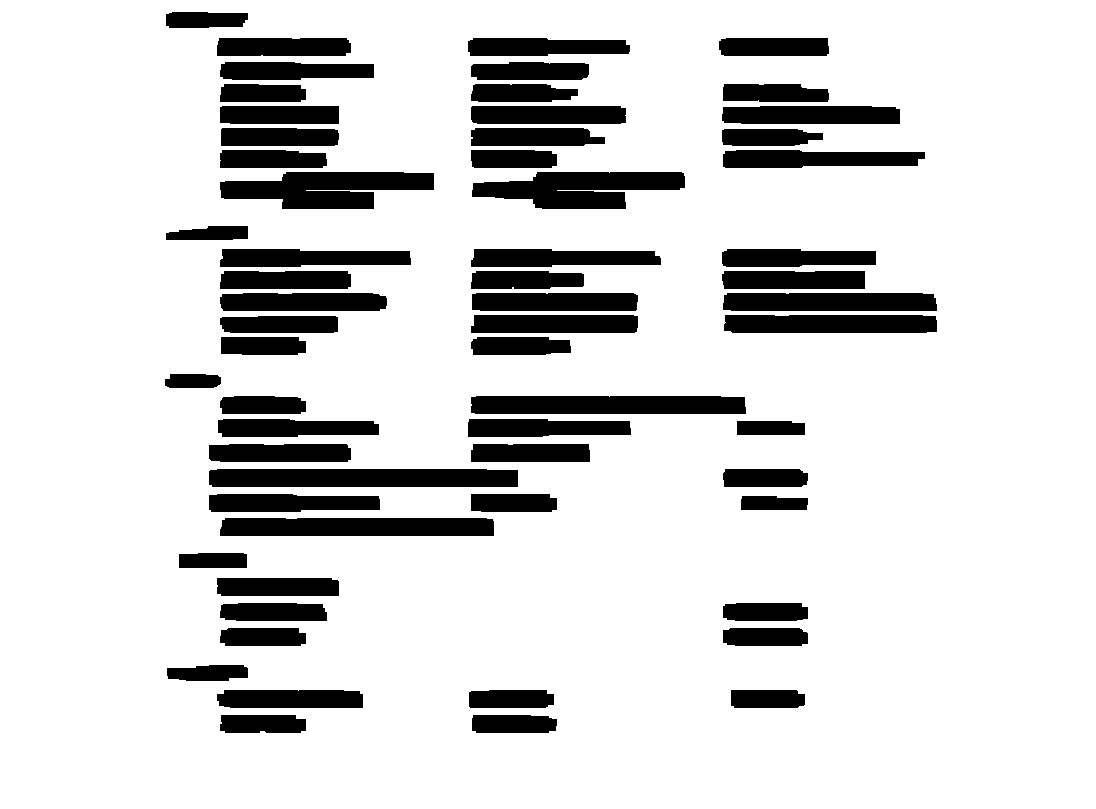
\includegraphics[width=\textwidth]{bingli1-cut-eroded}
  \end{minipage}
  }
	\hfill
  \subfloat[变换后的版式2]{
  \label{pic:bingli2-cut-eroded}
  \begin{minipage}[t]{0.23\textwidth}
    \centering
    
\includegraphics[width=\textwidth]{bingli2-cut-eroded}
  \end{minipage}
  }
  \subfloat[变换后的版式3]{
  \label{pic:bingli3-cut-eroded}
  \begin{minipage}[t]{0.23\textwidth}
    \centering
    
\includegraphics[width=\textwidth]{bingli3-cut-eroded}
  \end{minipage}
  }
	\hfill
  \subfloat[变换后的测试图]{
  \label{pic:new-bingli1-cut-eroded}
  \begin{minipage}[t]{0.23\textwidth}
    \centering
    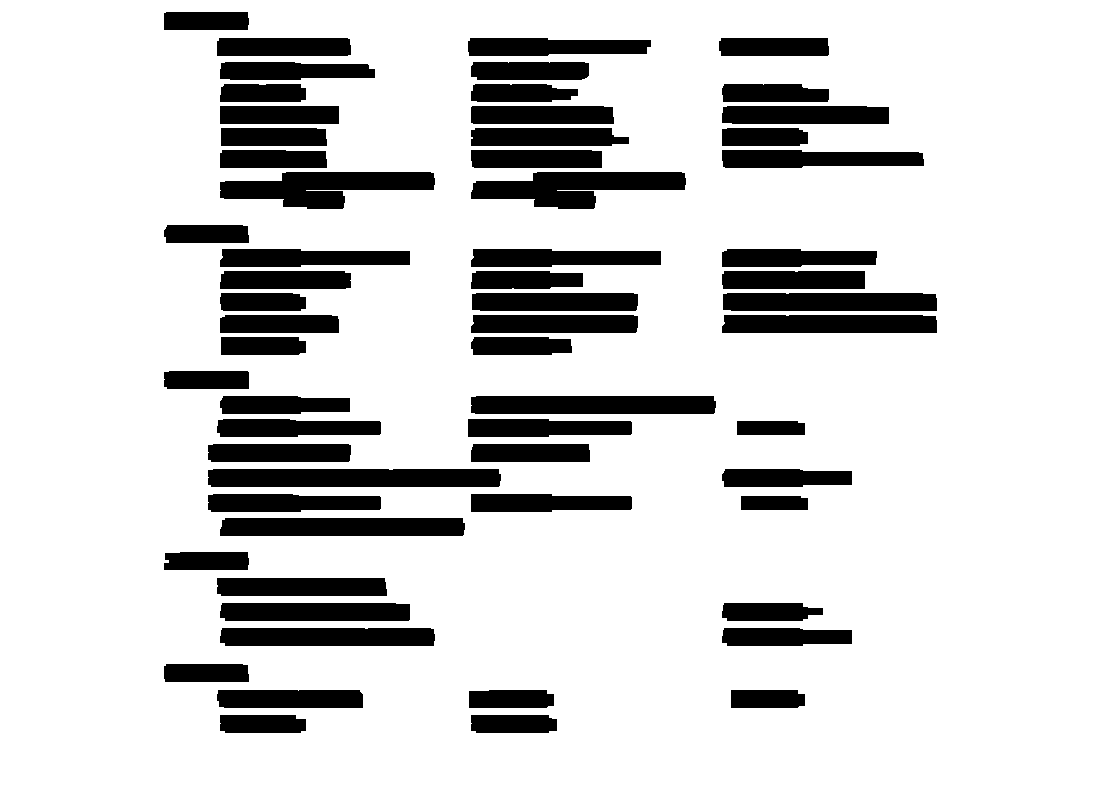
\includegraphics[width=\textwidth]{new-bingli1-cut-eroded}
  \end{minipage}
  }
  \caption{测试图片与模板图片的比较}
  \label{pic:layout-comparison}
\end{figure}

此时,这四张图片的信息比较复杂,字段中的文字实际上是判断版式的噪声,因此,我们将每张图片分别进行灰度化、二值化、腐蚀等转换操作,得到对应的\autoref{pic:bingli1-cut-eroded}、\autoref{pic:bingli2-cut-eroded}、\autoref{pic:bingli3-cut-eroded}、\autoref{pic:new-bingli1-cut-eroded}。经过转换后,图片都被二值化,即图片中的像素值只有0和1两种可能,0代表黑色,1代表白色。

每张图片我们都可以看成是一个矩阵,矩阵中的每个值要么是0,要么是1,我们采用的相似性度量指标为两张图(即两个矩阵)的点乘,显然,点乘的结果越大,说明两个图片中对应像素同时为1的像素点越多,也就可以认为越相似,点乘结果如\autoref{tab:dot-multy}所示,测试图片与版式1的点乘结果最大,因此可以认为测试图片的版式就是版式1。
\begin{table}
	\tabcaption{测试图与版式图的点乘结果}
	\label{tab:dot-multy}
	\centering
	\vspace{10pt}
  \renewcommand\arraystretch{1.5}  %这两行代码用来调整表格高度
	\begin{tabular}{|c||c|c|c|}
		\hline
		&版式1&版式2&版式3\\
		\hline
		点乘结果&$1.43\times 10^{11}$&$1.19\times 10^{11}$&$1.26\times 10^{11}$\\
		\hline
	\end{tabular}
\end{table}

但是我们可以看到,测试图片与各种版式的点乘结果间差距其实并不大,这样的判断指标显示不够有说服力,是什么原因造成点乘结果差距不明显呢?我们注意到,点乘结果主要计算的是对应像素同为1时的像素个数,即同时为白色的像素个数,而病历图片的大部分都被白色覆盖,导致点乘后,各个结果都比较接近,因此,我们可以将版式图片和测试图片的颜色都进行反转,即黑变白,白变黑,这样,点乘考量的就主要是图片中黑色相重叠的部分了。反转以后的点乘结果如\autoref{tab:dot-multy-reverse}所示,测试图片仍然是与版式1最接近,不过这一次,点乘结果间的差距更大了,这显然让我们更好做判断。

\begin{table}
	\tabcaption{测试图与版式图的反转点乘结果}
	\label{tab:dot-multy-reverse}
	\centering
	\vspace{10pt}
  \renewcommand\arraystretch{1.5}  %这两行代码用来调整表格高度
	\begin{tabular}{|c||c|c|c|}
		\hline
		&版式1&版式2&版式3\\
		\hline
		反转点乘结果&$2.62\times 10^{10}$&$1.04\times 10^{10}$&$0.95\times 10^{10}$\\
		\hline
	\end{tabular}
\end{table}

至此,我们已经完成了一张图片与版式图片之间的匹配,找到了最接近的版式,这也就意味着我们的图片分类工作完成了。

\subsection{字段提取}
接下来是版面分析的最后一步,字段提取。待分析的图片如\autoref{pic:bingli1_contours_origin}所示,我们观察可知,图片中每个字段相对于其他字段都有一定的距离,这使我们很自然的想到的通过连通域分析方法来进行字段提取工作。
\begin{figure}[htbp]
  \centering
  \subfloat[]{
  \label{pic:bingli1_contours_origin}
  \begin{minipage}[t]{0.3\textwidth}
    \centering
    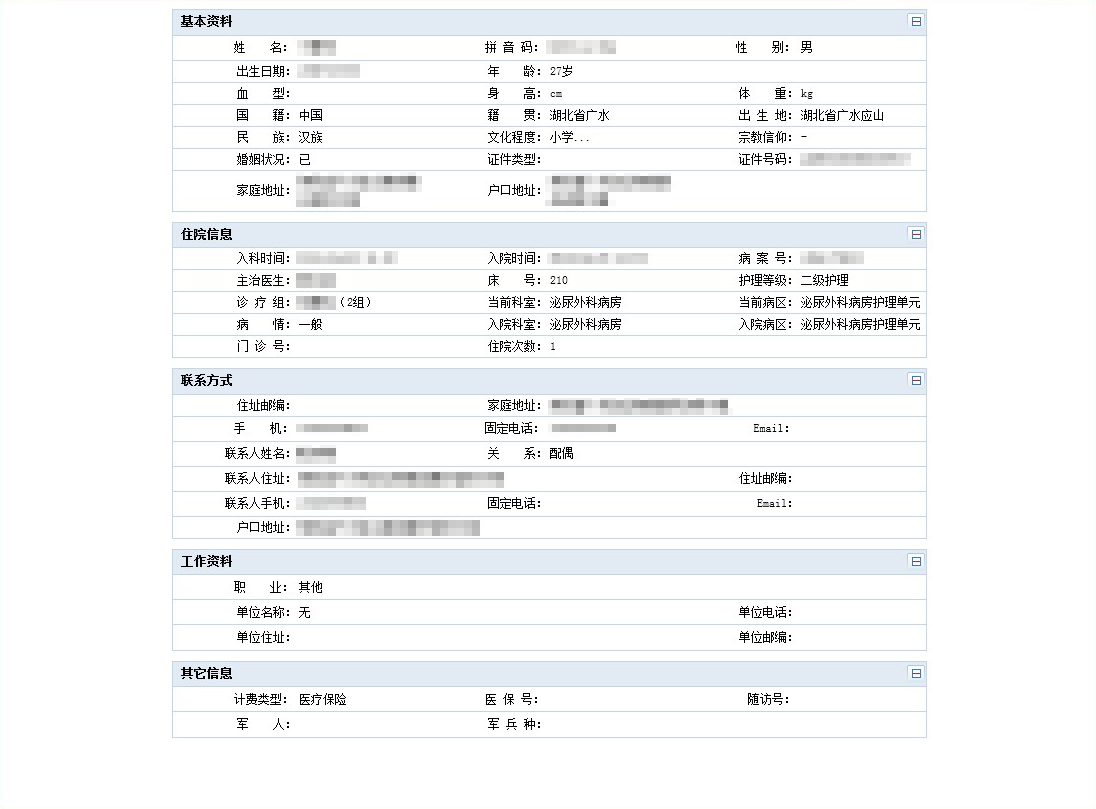
\includegraphics[width=\textwidth]{cut_sidebar}
  \end{minipage}
  }
  \subfloat[]{
  \label{pic:bingli1_contours_eroded}
  \begin{minipage}[t]{0.3\textwidth}
    \centering
    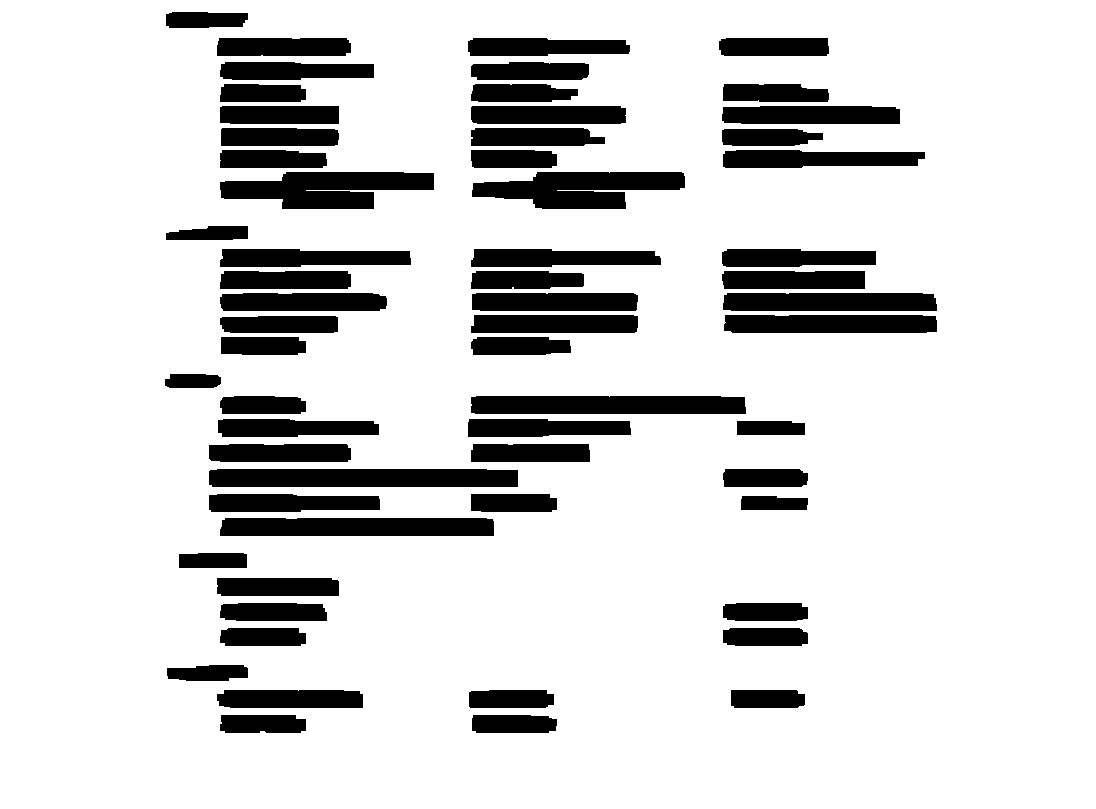
\includegraphics[width=\textwidth]{bingli1-cut-eroded}
  \end{minipage}
  }
  \subfloat[]{
  \label{pic:bingli1_contours}
  \begin{minipage}[t]{0.3\textwidth}
    \centering
    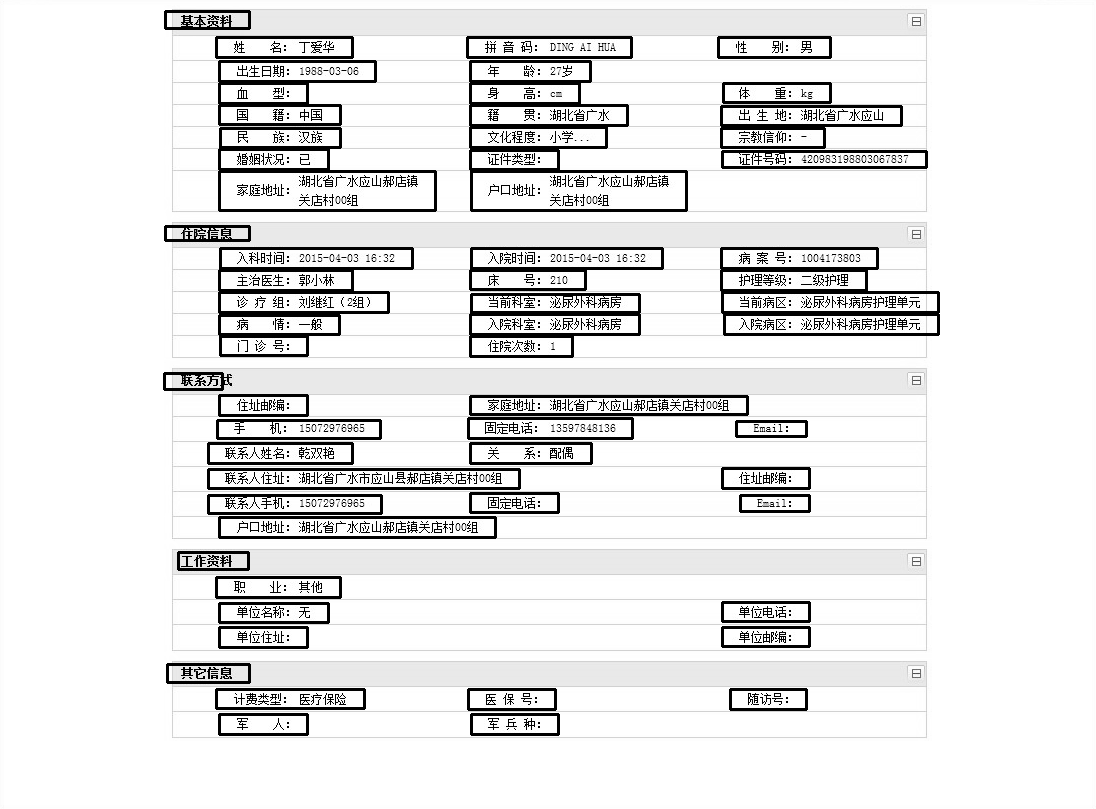
\includegraphics[width=\textwidth]{bingli1-contours}
  \end{minipage}
  }
  \caption{图片连通域分析}
  \label{pic:connected-component-analysis}
\end{figure}
连通域分析(Connected Component Analysis),是图像处理中一种常见的图片分割方法,顾名思义,它的主要作用是找到一张图片中(一般为二值图)连通的若干个子区域,并将它们从原图中划分出来,连通域分析方法在图像处理中有着广泛的应用,如人脸识别\citep{kuchi2002human},场景文字检测(Scene Text Detection)\citep{koo2013scene},网络中的社群发现(Community Detection)\citep{duch2005community}等等。另外,也有许多工作致力于快速地进行连通域分析,如优化两遍扫描法\citep{wu2009optimizing},线性时间连通域分析\citep{suzuki2003linear},并行化连通域分析\citep{han1990efficient}等等。

最常见的连通域分析方法有两遍扫描法(Two-Pass)和种子填充法(Seed Filling),两遍扫描法通过扫描两遍图像,获得全图的连通域信息并标注出来,而种子填充法则是先选取一个像素点作为种子(初始连通域),每次迭代都将与连通域相邻的像素纳入,知道找到所有属于同一连通域的像素集合,构成最终的连通域,然后重新选取种子确定下一个连通域,直到所有的连通域被找到,算法终止。在OpenCV中也内置了连通域分析函数。

我们注意到,在病历图片中,虽然字段间有一定的间隔,但字与字之间,甚至是字的内部,很多都是不连通的,如果我们直接对\autoref{pic:bingli1_contours_origin}进行连通域划分,效果会很差,因此,需要对原图片进行与前一小节类似的灰度化、二值化、腐蚀等处理,将字内部、字与字之间都连接起来,同时保持字段的分隔,\autoref{pic:bingli1_contours_origin}经过这一系列转换,我们得到如\autoref{pic:bingli1_contours_eroded}所示的二值化腐蚀图像,然后对它进行连通域分析,再将找到的连通域位置映射到原图,就得到\autoref{pic:bingli1_contours},我们看到,各个字段被矩形框框住,同时字段与字段之间很好的分隔开了,字段提取工作完成。

至此,我们完成了版面分析的全部工作。

\section{预处理模块}     % 1000字
虽然原始的病历图片并不算模糊,但是由于每个字相对来说很小,导致当我们将截取出来的字段放大来看时,每个字的笔画很模糊,有不少噪声,并且像素化明显(见\autoref{pic:image-before-processing},这是从病历图片中截取出来的一个字段),这样的文字对于文字识别来说是很困难的,因此我们需要一个预处理模块,来对文字进行放大,加粗线条,去除噪声,降低识别难度。
首先要做的就是文字的放大,在放大的过程中,为了保持文字的连贯,避免由于文字笔画太细出现中断的情况,我们需要用到插值(interpolation)算法。插值算法在图像处理领域有着广泛的运用\citep{thevenaz2000image},简单来说它是一种根据已有像素点的值来填充新像素点的方法,常用的插值方法有以下几种:
\begin{itemize}
	\item 最近邻插值,这是一种最简单的插值算法,新像素点的值由离它最近的像素点确定,即与最近的像素点的值保持一致,显然这样的话,图片会有比较明显的锯齿效应。
	\item 线性插值,是指以线性函数为插值函数的插值方法,对于最简单的一维情况,它的数学表达式可写为
		\begin{equation}
			P(x) = f_0\frac{x-x_1}{x_0-x_1}+f_1\frac{x-x_0}{x_1-x_0}
		\end{equation}
		其中,$x_0$、$x_1$分别为已知的两个像素点的坐标,$f_0$、$f_1$为它们对应的像素值,那么新像素点$x$的像素值为$P(x)$。
	\item 双线性插值,它可以被看做是线性插值的一个拓展,核心思想是在两个方向上各进行一次线性插值,叠加结果得到新像素点的像素值。
\end{itemize}
除此之外,还有双三次插值、分形插值(Fractal Interpolation)\citep{barnsley1986fractal}、边缘定向插值(Edge-directed Interpolation)\citep{li2001new}等,这里就不再一一介绍。
OpenCV中进行图片放缩的时候,支持指定自带的几种插值方法,函数原型是:
\begin{Code}
void resize(InputArray src, OutputArray dst, Size dsize, double fx=0, double fy=0, int interpolation=INTER_LINEAR )
\end{Code}
其中最后一个参数,用来指定插值方法,支持最近邻插值、双线性插值、双三次插值等。

文字经过二值化、放缩等步骤以后,最后转换成了\autoref{pic:image-after-processing},可以看到,相比于原图,图片更加纯净,去除了大量的早点,同时文字线条也更加饱满清晰,更加便于文字识别系统的识别,后续的实验也证明这大大提高了文字识别精度。至此,图片的预处理阶段完成。
\begin{figure}[htbp]
  \centering
  \subfloat[]{
  \label{pic:image-before-processing}
  \begin{minipage}[t]{0.45\textwidth}
    \centering
    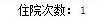
\includegraphics[width=\textwidth]{text-origin}
  \end{minipage}
  }
	\hfill
  \subfloat[]{
  \label{pic:image-after-processing}
  \begin{minipage}[t]{0.45\textwidth}
    \centering
    
\includegraphics[width=\textwidth]{text-resized}
  \end{minipage}
  }
  \caption{文字的预处理}
  \label{pic:pre-processing}
\end{figure}

\section{OCR模块}     % 6000字
在前面的章节中,我们已经简要介绍了开源OCR引擎Tesseract的发展历史和基本现状,作为整个系统的核心模块,我们有必要对Tesseract有更加详细的了解,接下来,我们将从架构、实现细节方面来展开介绍。这部分内容主要参考自Tesseract的开发者Ray Smith的两篇文章\autoref{smith2007Tesseract,smith2013history}以及部分Tesseract的源码\footnote{Tesseract源码可见:https://github.com/tesseract-ocr/tesseract}。

\subsection{整体流程}
首先要说明的是,由于惠普公司当时在开发这套系统的时候,使用的是公司内部固定的版式,因此,从一开始Tesseract就不需要自己的版面分析系统,因此,Tesseract默认假设输入的图片数据是已经二值化的只包含若干个文本区域的图片数据。整个处理流程是比较传统的逐步管道模式(step-by-step pipeline)。

第一步是进行连通域分析,同时将识别出来的连通域轮廓保存下来,这在当时是一个计算消耗比较大的设计,不过也赋予了Tesseract一个特别的优势:通过检查嵌套的轮廓,以及子轮廓的数目,此时,文字的全部信息都被存到文字的轮廓中,已经剥离了文字的颜色信息,因此它能很容易的进行反转文字(inverse text)的识别,即“黑底白字”的识别。Tesseract被认为是首个具有比较强的翻转文字识别能力的OCR引擎。这些嵌套的轮廓聚合在一起,构成若干个文字块(Blobs)。

第二步是将这些文字块组成一行行文字,它们会根据不同的字符间距(character spacing)被划分为一个个单词。定宽(fixed pitch)的文字,会根据字符单元格(character cells)被直接划分切分成词,而不定宽(proportional)的文字则会根据绝对间距(definite spaces)和模糊间距(fuzzy spaces)来切分成词。

第三步就是文字识别。它是一个两遍(two-pass)识别过程,在第一遍时,识别系统会尝试着轮流识别每个单词。每当识别一个有可信度的单词时,这个单词就会被加入到一个自适应分类器(adaptive classifier)中,作为训练数据。这样这个自适应分类器就能在识别接下来的文字时有更高的精度。如果只过一遍网络,那么自适应分类器学到的新知识就无法应用到当前的文本中,因此,需要过第二遍识别,这一次识别的重点是第一遍中没有能够很好识别的那些文字。

最后一步处理模糊间距,检查其他可能的字体高度划分方法。

\subsection{重要细节}
上一小节,我们粗略地介绍了Tesseract的整体识别流程,帮助我们宏观地了解Tesseract的架构,接下来,我们会总结一些影响到Tesseract性能的重要细节。

\subsubsection*{缺乏版面分析能力}
就像这一节刚开始提到的那样,由于Tesseract最开始由惠普公司开发的时候,只针对惠普公司内部的特定版式,所以,它在设计之初就没有任何版面分析的模块(这也是为什么在整体流程中没有版面分析这一步),因此,Tesseract只能作为一个识别确定文本区域的文字识别模块,它的输出也只局限于文本,并没有关于版式的信息。在处理特定任务时,我们往往需要根据问题特点,自己设计实现版面分析功能,这也就是为什么很多类似于Tesseract这样的文字识别引擎不能直接用于复杂的文字识别任务。

\subsubsection*{多语言支持}
最初的Tesseract只支持英文的识别,到了Tesseract 2.0版本,加入了Unicode(UTF-8)的支持,此时支持的语言达到6种,而到了Tesseract 3.0版本,又增加了多种新语言支持,这其中就包括中文、日语、韩语。如今,它支持的语言已经将近90种,并且支持同时在一张图中识别多种语言。这些语言各不相同,每种语言都有数千种不同的形状,如果Tesseract要同时支持如此多种语言的话,字符匹配的难度无疑会大大增加,并且这种大而全的文字识别器其实并不实用,大多数情况下,需要识别的文字可能只是其中特定的一到两种,其他语言的引入反而是极大的干扰。那么Tesseract是如何做到多语言支持的同时又保证实用性呢?答案是它支持用户自定义训练集,也就是说,用户可以根据需求只将需要识别的语言加入到训练集中,让识别精度得到了有效保障。

\subsubsection*{异常字符确定}
在以中文字符为主的文本块中,偶尔会出现一些英文字符,数字,标点符号等,怎么确定哪些符号是非中文字符(或异常字符)呢?这里有一个很重要的先验知识,那就是这些异常字符一般与正常的中文字符在高度上是不一致的,如\autoref{pic:image-after-processing}中,“住院次数”在字符高度上明显比数字“1”要高,那么,当我们大体确定了整行或整篇文字的平均高度以后,那些低于平均高度的字符,就可以高可信地认为是异常字符(即英文、数字、标点等),这样我们相当于对数据做了一次划分(中文与非中文),减少了各自类型字符识别的可能情况,从而提高了识别精度(尤其是对异常字符)。

\subsubsection*{不等宽单词的划分}
不等宽单词的划分是识别中的一个难点,如\autoref{pic:difficult-word-spacing}中所示的单词“of”和“financial”,如果我们用两个边界框(bounding box)将它们框起来的话,会发现这两个单词之间并没有任何横向间隔(horizontal gap),意即计算机系统是无法根据边界框来将这两个单词划分出来的,但是人却能很明显地将它们区分开来,为什么呢?一个比较有说服力的解释是我们是从两个两个单词的中线部分能明显看到间隔。Tesseract也是利用了这个知识,在处理不等宽单词的划分时,它考量的是单词在基线(baseline)与中线(mean line)之间的某个区域内的间隔,这样就能将它们很明确的划分开来。
\begin{figure}
	\centering
	
\includegraphics[width=0.5\textwidth]{difficult-word-spacing}
	\caption{不等宽单词的划分}
	\label{pic:difficult-word-spacing}
\end{figure}

\subsubsection*{分类器候选词}
文字识别分类器在识别过程中,会给出某个待识别单词的一系列可能的候选词,以及每个候选词的置信度得分(confidence scores),之后再结合字典、前后文信息等,得到综合得分,然后选取得分最高的单词作为最后的识别结果。这个置信度得分会在切分粘连字符时用到。

\subsubsection*{粘连字符的切分}
有时候由于预处理是文字的放缩失当,会导致部分字符粘连在一起,如\autoref{pic:chopping-joint-characters}中所示单词“arm”就被粘连在一起,这样势必导致识别置信度较低,此时,Tesseract会尝试对粘连字符(置信度得分低的字块)进行切分,切分的候选点是所有轮廓多边形的凹点(concave vertices),即\autoref{pic:chopping-joint-characters}中小三角形标注的点,Tesseract会逐一按照各个凹点进行切分,重新识别,只保留置信度较高的切分方式,这样,就能正确地将三个字母正确切分出来。
\begin{figure}
	\centering
	
\includegraphics[width=0.5\textwidth]{chopping-joint-characters}
	\caption{粘连字符的切分}
	\label{pic:chopping-joint-characters}
\end{figure}

\subsubsection*{不同划分方法的比较}
对于同一段文本块,它即可能被划分为$A$、$B$两个单词,也有可能被划分为$C$、$D$、$E$三个单词,这时如何比较两种划分的优劣呢?如果简单的将两边每个单词的置信度相加比较肯定是不当的,因为第二种划分有3个单词,置信度相加以后的和很可能会比只有两个单词的置信度之和要大;那么将置信度之和除以单词数目之后再比较呢?这种均分置信度也有问题,因为各个单词的长度并不相等,各自在整个文本块中所占的“比重”并不一样,直接平均也不可取。因此,最终采用的计算方案如\autoref{eq:confidence-comparison}所示,由于同一段文本块的总长度$len$一定,每个单词的置信权重取决于它在整个文本块中的“比重”。
\begin{equation} \label{eq:confidence-comparison}
	\begin{split}
		&Conf(AB) = Conf(A)\frac{Len(A)}{len} + Conf(B)\frac{Len(B)}{len} \\
		&where \quad len=Len(A) + Len(B)
	\end{split}
\end{equation}

\subsubsection*{自适应分类器}
在Tesseract中,有两个分类器:静态分类器(static classifier)和自适应分类器(adaptive classifier)。由于静态分类器涉及到多种字体,通用性比较强,但是其区分相近字符、字符与非字符的能力被削弱。此时,由于每页文档内的字符的个数有限,利用静态分类器的结果可以训练出对字体更敏感的自适应分类器,可以提高分类能力。%这几句摘自http://blog.csdn.net/viewcode/article/details/7790065
Tesseract在识别时会做两遍识别,第一遍时,识别系统会尝试着轮流识别每个单词。每当识别一个有可信度的单词时,这个单词就会被加入到一个自适应分类器(adaptive classifier)中,作为训练数据。这样这个自适应分类器就能在识别接下来的文字时有更高的精度。如果只过一遍网络,那么自适应分类器学到的新知识就无法应用到当前的文本中,因此,需要过第二遍识别,这一次识别的重点是第一遍中没有能够很好识别的那些文字。%这几句与“整体流程”小节一样。
因此,自适应分类器让Tesseract具有了即时(on-the-fly)的学习能力。

\subsubsection*{分类器模型}
Tesseract中采用的分类器模型是k近邻(k-Nearest Neighbour,KNN),采用的距离度量是在特征空间里的欧几里得距离,k近邻是机器学习中比较成熟的分类模型,它的核心思路是:如果一个样本在特征空间里面k个最相似的样本中的大多数属于某一个类别,那么该样本也属于这个类别。k近邻虽然实现简单,但是它有 一个很大的缺点就是计算量比较大,因为每个样本需要与其他所有的样本进行距离计算,当特征空间维数大或者训练数据容量大时,无疑是非常耗时的。这也是Tesseract在识别速度上不如市面上很多商业化OCR软件的原因之一。
另外,Tesseract为了支持阿拉伯语专门实现了一个卷积神经网络(Convolutional neural networks,CNN)分类器,在阿拉伯语上表现很好,但在欧洲语言上,性能和效果都不行。%这一句摘自http://zhuanlan.zhihu.com/p/20231514

\subsection{字符库训练}
Tesseract官方提供了一个中文字符库\footnote{官方提供的多种语言字符库下载:https://github.com/tesseract-ocr/tessdata},用来对中文进行识别,这个字符库中包含了印刷体中文里的很多种字体,是一个大而全的字符库,

\subsection{添加用户字典}


\section{字段解析模块}  %3000字
当含有文本的图片数据经过OCR模块以后,会被转换为文本,这些文本需要进行一定的加工,才能得到我们想要的各字段数据。总体来说,原始的文本需要经过数据清洗、字段匹配、目标文本提取等步骤。我们也可以认为这是数据的“后处理”过程。

\subsection{数据清洗}
数据清洗主要有两大功能,一是对文本的冗余信息(如因为图片噪声而产生的冗余符号)进行剔除,二是对文本进行简单的矫正。这两部分实现难度不大,却对之后的字段匹配过程有着很大的帮助。
\subsubsection{冗余信息剔除}
\subsubsection{文本矫正}

\subsection{字段匹配}
某段文本属于哪一个字段呢?这就需要对文本的具体内容进行理解划分了,例如若要判断
\subsubsection{StartsWith匹配}
\subsubsection{Includes匹配}


\section{数据存储模块} %500字

\section{小结}
 %第四章,实现细节   17000
  \chapter{实验}
\label{chap:experiments}
 %第五章,实验   3000
  \chapter{结论}
\label{chap:conclusion}
\section*{总结}
本文首先介绍了病历档案自动归档与分类系统的研究背景和意义,从实际应用场景出发,深入分析并明确了系统的各项功能和性能需求。
在此之上,本文设计了一个多模块、松耦合的流水线式的系统整体框架,使得系统具有高效、高扩展性的特点。
在实现细节上,系统基于开源图片处理库OpenCV和开源字符识别引擎Tesseract,加入版面分析、医疗数据训练集、数据预处理和后处理等的支持,实现了一个针对真实应用场景的印刷体病历档案自动归档与分类系统。
实验证明,系统在版面分析、字段提取、文字识别等方面都有着较高的准确率,具备较高的可靠性和实用价值。

本文核心工作可以归纳为:
\begin{itemize}
  \item 针对特定的病历图片数据,通过图像处理技术,设计和实现了完善的版面分析模块,填补了大部分商用OCR软件应用到病历数据时在版面分析能力的缺失。
  \item 基于开源OCR引擎Tesseract,针对病历数据,增加了图片预处理、医疗数据训练集、文本后处理等的支持,大大提高了文本识别的准确率。
\end{itemize}

\section*{后续工作}
对于医学档案自动归档与分类系统来说,最核心的性能指标就是识别准确率和处理速度。
在系统开发和测试过程中,本系统的文字识别准确率和处理速度虽然都达到了预期的设计要求,但是都有一定的提升空间。
在后续的工作中,将从这两方面来提升系统的性能。
\subsection*{准确率提升}
虽然Tesseract支持加入用户字典,来加强对高频词的识别准确率,但是从实验中可以看到,用户字典的加入对于性能的提升很有限,说明Tesseract在字典信息的利用上并不是很优秀,本系统可从这方面着手提高识别准确率。

事实上,Tesseract提供了识别候选字接口,即对于每个字,Tesseract在识别过程中会产生多个候选字,并给出每个候选字的置信度,再根据上下文信息,用户字典等,给出每个候选字的综合打分,保留综合得分最高的字作为最后的输出。
那么,一个可能的优化方案是系统拿到各个字的识别候选字及其置信度以后,根据统计语言模型(Statistical Language Modeling)\citep{brown1990statistical}建模,得到最可能的候选字组合,这种方法也许能有效提高文字识别准确率。
\subsection*{速度提升}
从实验中可以看到,本系统在处理速度上主要受限于Tesseract的文字识别速度,其他模块的优化提速并不会明显提高系统的整理处理速度。
一个简单可行的提升方法是将本系统部署到多机环境中,只要做好数据读取和存储时的协同,理论上处理速度会随着机器数目线性增长。
 %第六章,结论 1000

  %
\chapter{绪论}
\label{chap:introduction}

中国科学技术大学论文模板(ustcthesis)是按照中国科学技术大学学士、硕士和博士论文要求制作的\LaTeX 通用论文模板。其前身是中国科学技术大学本科论文模板(作者XPS,最后维护ywg)和中国科学技术大学研究生论文模板(作者Liuqs,主要维护Liuqs、Guolicai)。本模板在上述两模板基础上进行了整合梳理,将模板的基础实现和增强功能进行分离,分别提供最基础的ustcthesis.cls以及增强包ustcxtra.cls。其中,ustcthesis.cls仅提供模板的最基础格式,ustcxtra.cls则包含一些常用的优化设置及更为便捷的自定义命令。

本文是使用上述模板生成的示例文档,目的在于帮助使用者熟悉该模板的使用方法,并且为使用者学位论文的撰写提供基础代码示例。

\section{系统要求}
\subsection{系统要求}
本模板基于\CTeX 的ctexbook文档类进行定制,基于\XeTeX 引擎排版。使用本模板的最基础功能时,除了上述需求外,还需要如下几类宏包(直接引用):
\begin{description}
\item[数学类]{amsmath、amsthm、amsfonts、amssymb、bm}
\item[格式类]{titletoc、titlesec、geometry、caption}
\item[表格类]{multicol、multirow}
\item[其他]{xparse、xeCJK、hyperref、natbib、subfiles}
\end{description}
可能有部分宏包是由上述宏包以及\CTeX 间接引用的,此处不一一列举。

另外,如果需要使用增强的ustcxtra.cls,额外需要如下宏包(直接引用):
\begin{description}
\item[默认载入]{times、algorithm2e、graphicx、psfrag、subfig、enumerate、epsfig、float、paralist、booktabs、footmisc、wasysym、longtable、bbm、indentfirst、ifthen、caption3、array、fancyvrb、xcolor、url}
\item[条件载入]{eulervm(仅在文档类处于增强模式并在文档类选项注明euler时载入)}
\end{description}

\section{下载与安装}
\subsection{模板文件清单}
使用模板之前请确保模板文件没有缺失损坏。文件清单如\autoref{tab:filelist},标注关键的文件需要确保文件以及路径的完整。
\begin{table}[htp]
\centering
\tabcaption{模板主要文件清单}
\label{tab:filelist}
\begin{tabular}{lll}
\toprule
文件名&相对路径&备注\tabularnewline
\midrule
clean.bat			&./			&清理脚本\tabularnewline
clean.sh			&./			&清理脚本\tabularnewline
main.pdf			&./			&示例文件\tabularnewline
main.tex 			&./			&示例TeX文件\tabularnewline
make.bat			&./			&生成脚本\tabularnewline
make.sh				&./			&生成脚本\tabularnewline
ustcbib.bst		&./			&Bib格式文件\tabularnewline
ustcthesis.cls		&./			&(关键)模板\tabularnewline
ustcxtra.cls		&./			&(关键)模板增强\tabularnewline
ustc\_logo\_fig.eps	&./figures	&(关键)科大校徽\tabularnewline
ustc\_logo\_text.eps&./figures	&(关键)科大校名\tabularnewline
\bottomrule
\end{tabular}
\end{table}

\subsection{模板下载与使用}
由于Google公司决定停止Google Code服务,故原Google Code项目网站的模板整体迁移至GitHub网站并继续进行更新维护。本模板及本示例文件可以在GitHub网
站\url{https://github.com/ywgATustcbbs?tab=repositories}下载。备份托管地址为\url{https://gitlab.lug.ustc.edu.cn/ywg/ustcthesis},此托管网站由LUG@USTC提供服务。

请在项目页面选择ustcthesis->新页面中选择Download Zip下载最新模板文件(\autoref{fig:download})。也可以通过git clone的方式获得模板。

\begin{figure}
\centering
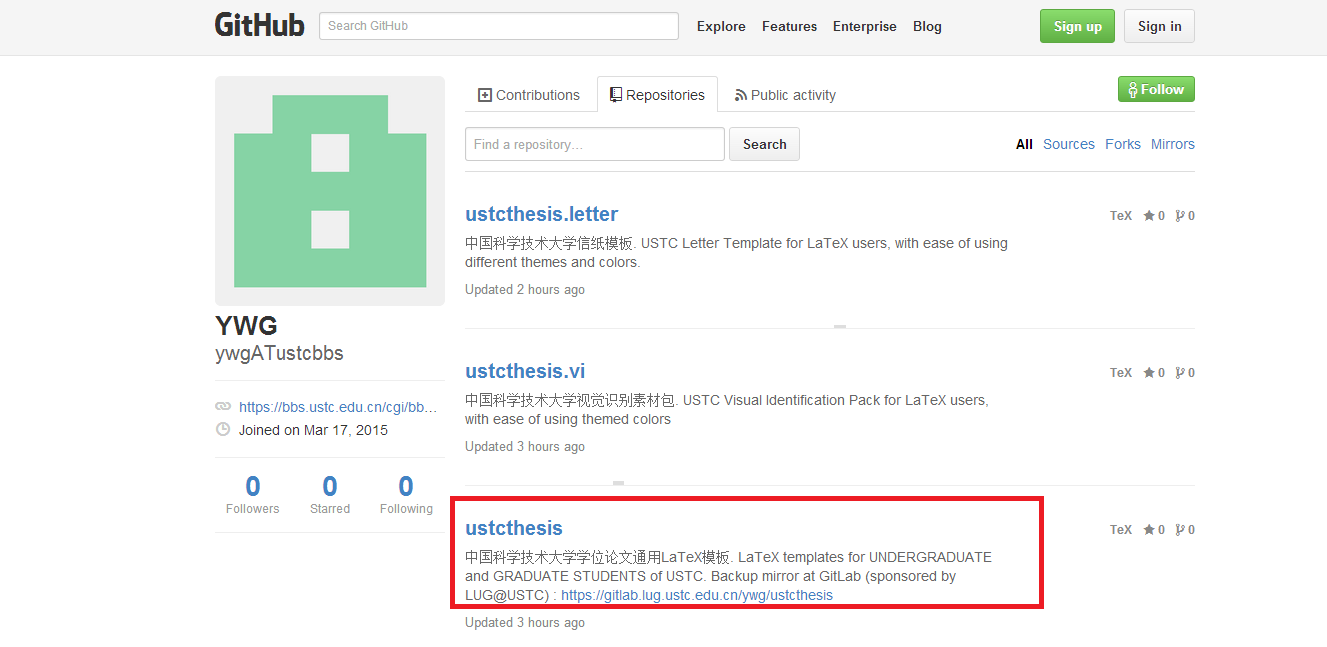
\includegraphics[width=0.48\textwidth]{download}
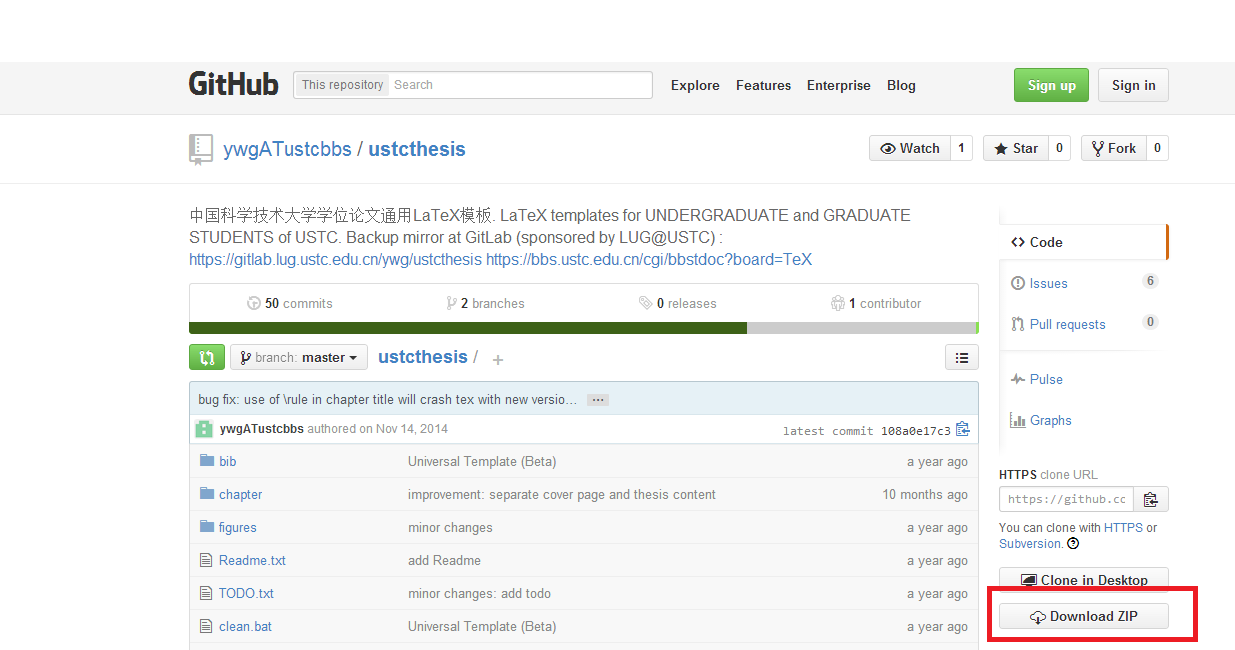
\includegraphics[width=0.48\textwidth]{download1}
\figcaption{在GitHub上进行模板下载}
\label{fig:download}
\end{figure}

\textbf{特别注意1:}本硕博通用论文模板的名称为ustcthesis,其他项目如ustcthesis.vi/ustcthesis.letter/ustcthesis.beamer是用作其他用途的模板,并非本模板所需文件,如对其感兴趣,请进入对应页面了解详情。

\textbf{特别注意2:}此前开发的本科和硕博模板已暂停支持,但仍然可以选择对应的版本(ustcthesis.bachelor和ustcthesis.msphd)进行下载。

模板的安装使用方法有多种,最为简单便捷的方法是直接解压缩下载好的压缩包,修改其中的main.tex文件以及chapter文件夹下的文件,必要时增加所需要的文件。需要注意的是确保所有文件使用UTF-8编码。Windows系统中将其他编码的文件转化为UTF-8的方法是: 用记事本打开这些文件, 然后点击文件—另存为—在最下方选择UTF-8 编码。

\subsection{\texorpdfstring{\LaTeX}{LaTeX}系统的安装和使用}
由于本模板使用了较多的宏包,因此建议使用TeXLive2013及以上版本的\LaTeX 发行版。TeXLive2013可以在Windows、GNU/Linux和大多数Unix系统中运行。对于MacOSX,推荐使用MacTeX-2013。详细信息参考\url{https://www.tug.org/texlive/}。

对于中国科学技术大学的校内用户而言,最方便的获取TeXLive2013的途径是使用LUG@USTC提供的CTAN镜像源(\url{http://mirrors.ustc.edu.cn/CTAN/})。最新的TeXLive位于/CTAN/systems/texlive/目录(\url{http://mirrors.ustc.edu.cn/CTAN/systems/texlive/})内。用户可以选择进入Images文件夹下载完整的光盘并刻录安装,也可以选择进入tlnet文件夹下载运行install-tl.exe进行在线安装。需要注意的是,在线安装的时候可以通过切换安装源为本校镜像源来加快下载安装速度。

对于校外用户,可以通过CTAN.org获得官方的TeXLive。CTAN在全球41个国家和地区分布有115个镜像站点,它们的地址可以在\url{http://www.ctan.org/mirrors/}找到。

\subsection{推荐使用的编辑器}
\LaTeX 的源文件是一个或多个文本文件,这意味着可以使用最为简单的文本编辑器来撰写论文。但是和许多编程语言类似,使用一款带有语法高亮、命令补全等功能的文本编辑器能够大大提升协作效率。

对于不同的编辑器而言,能够实现的功能也不尽相同,加之不同用户拥有不同的使用习惯,简单武断的说某一款编辑器好或者不好有失公允。对于\TeX 写作而言,用户使用的编辑器大致可以分为两类:通用的文本编辑器和专用的GUI编辑器。通用的文本编辑器中公认比较好用的有Vim(Linux)、Emacs(Linux)、Notepad++(Windows)等等\footnote{当然,这些软件可能都有跨平台版本,而且也有其他很多优秀的文本编辑器,不要在意这些细节啦,我并不想挑起编辑器的圣战。:P}。这些编辑器有着强大的功能,但是往往需要在编辑和编译之间来回切换。而专用的GUI编辑器如TeXShop(Mac)、TeXWorks(windows/Linux)和Winedit(Windows、付费软件)等虽然可能在文本编辑上略显笨拙,但是其优点在于编写和生成一体化,简单化。

使用何种编辑器这个问题见仁见智,但是对于一个刚从word转来的新人,从界面简洁、操作简单、功能实用的角度出发,TeXWorks不失为一款优秀的GUI软件,如\autoref{fig:texworks}。

\begin{figure}
\centering
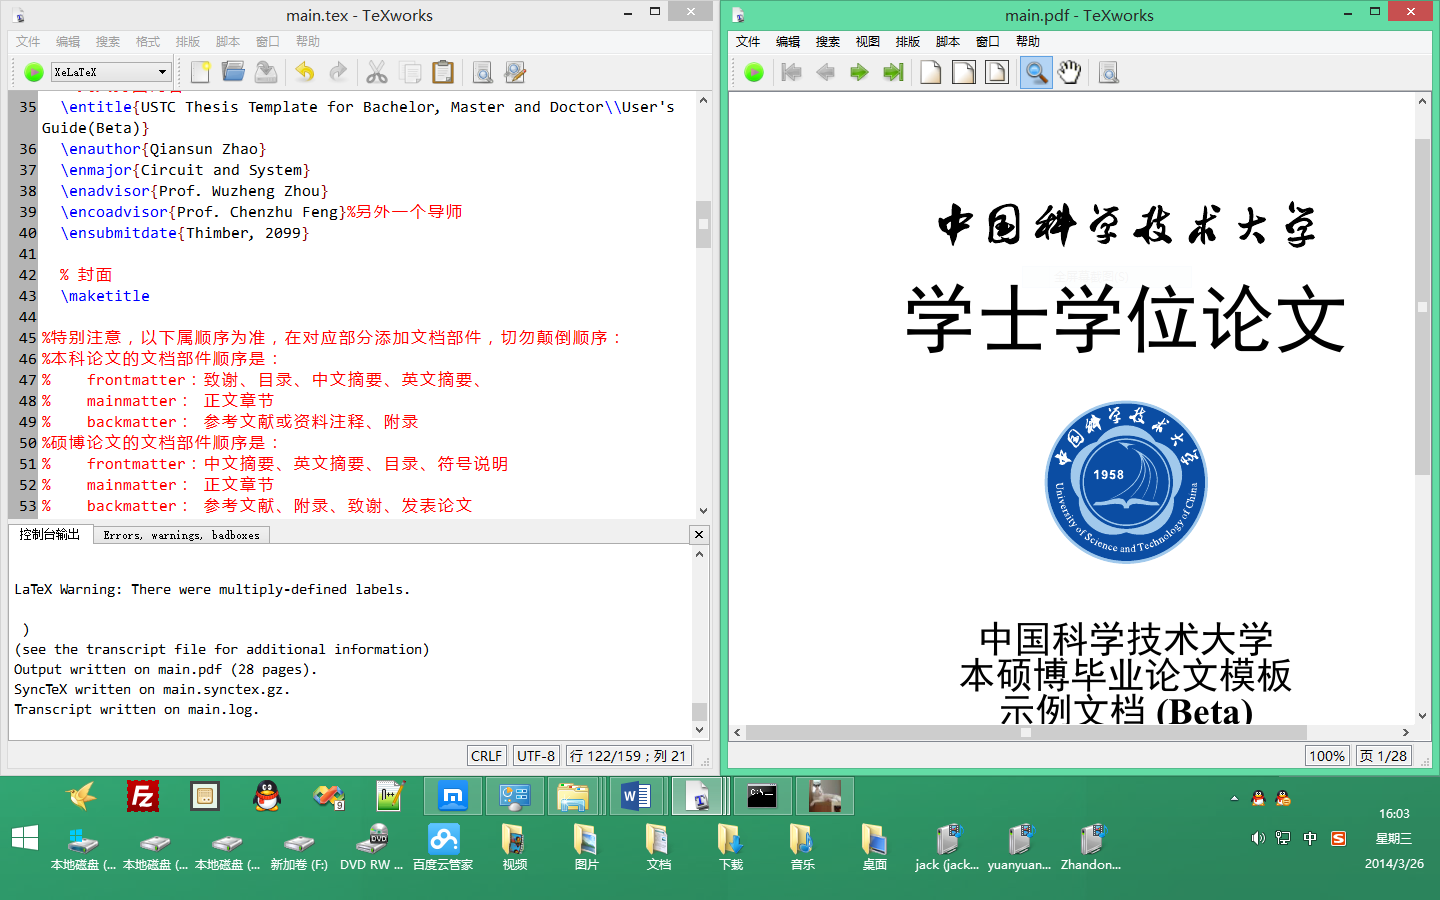
\includegraphics[width=0.9\textwidth]{texworks}
\figcaption{TeXWorks主界面}
\label{fig:texworks}
\end{figure}

Windows系统下TeXWorks的界面拥有左右两个窗口,左边为编辑窗口,右边为预览窗口,当编辑完文档之后,只需点击绿色的开始按钮,就可以立即对文档进行保存并编译,可以选择不同的引擎进行处理。编译过程中的信息会在左侧窗口下方显示。TeXWorks默认UTF-8编码,安装时自动查找TeX安装目录,支持自动缩进、语法高亮、命令补全、正则式查找以及TeX文件和PDF的正反查找(即点击命令跳转到对应pdf文字位置以及点击pdf文字跳转到对应命令,操作是Ctrl+单击)。这些功能对新手来说都是十分友好的。

\section{问题反馈}

如果您在使用过程中有疑问,遇到困难,可以在\href{http://bbs.ustc.edu.cn/cgi/bbsdoc?board=TeX}{瀚海星云\TeX{}讨论区}或者相关的\LaTeX 论坛(如\href{http://bbs.ctex.org}{CTEX 论坛})寻求帮助,但是请注意遵守论坛的各项规定。

如果使用过程中遇到Bug,请提交到\href{http://bbs.ustc.edu.cn/cgi/bbsdoc?board=TeX}{瀚海星云\TeX{}讨论区},或者提交到相应的\href{http://code.google.com/p/ustcthesis/issues/list}{Google UstcThesis Project(http://code.google.com/p/ustcthesis/issues/list)},请注明是什么版本模板的bug。
  %\chapter{模板的基础使用说明}

\section{模板基本说明}
使用本模板,您应首先具备基本的\LaTeX 知识,如果您刚刚接触\LaTeX,建议您先学习相关的用户文档或教程。

模板文件名为ustcthesis.cls。方便起见,将该文件放置在与论文主文件同一文件夹中即可。如果需要使用增强功能,模板提供了一个名为ustcxtra.cls的补充包。将该文件放置在与论文主文件同一文件夹中即可。

模板提供一个文档类ustcthesis,使用\verb|\documentclass{ustcthesis}|来加载模板。

模板可以使用ctexbook文档类的相应选项,默认加载的是 cs4size, a4paper, fancyhdr, fntef。需要注意的是默认加载 \emph{双面/章节从奇数页开始} 选项,如果需要\emph{单面} 选项,请使用:
\begin{Code}
\documentclass[<学位>,oneside,openany]{ustcthesis}
\end{Code}

\begin{table}[htp]
\centering
\tabcaption{模板提供的新文档选项}
\label{tab:newdocopt}
\begin{tabular}{lL{5cm}L{4cm}}
\toprule
文档选项&说明&备注\tabularnewline
\midrule
bachelor	&学士				&\multirow{3}{4cm}{指明论文类型,不能同时存在}\tabularnewline
master		&硕士				&\tabularnewline
doctor		&博士				&\tabularnewline
basic		&仅使用基础功能	&此时无法使用增强包中的命令\tabularnewline
oldfontcfg	&使用老版本的硕博论文模板的字体设置			&需要补充包\tabularnewline
euler		&使用euler数学字体&需要补充包\tabularnewline
adobefont	&使用adobe的字体	&\multirow{2}{4cm}{仅仅防止误输入}\tabularnewline
adobefonts	&使用adobe的字体	&\tabularnewline
notchinese	&使用外文撰写论文	Use this option to write thesis in other laguage(s)& If you use language(s) other than Chinese and English, you should refer to \autoref{tab:newcmd}. \tabularnewline
\bottomrule
\end{tabular}
\end{table}

\subsection{模板推荐加载设置}
推荐使用如下选项加载模板:
\begin{Code}
\documentclass[<学位>,euler,twoside,openright]{ustcthesis}
\end{Code}

如果缺少大多数宏包,建议使用
\begin{Code}
\documentclass[<学位>,basic,twoside,openright]{ustcthesis}
\end{Code}

\section{模板提供的新环境和命令}
模板提供了若干个新环境和命令,如\autoref{tab:newenv}和\autoref{tab:newcmd}所列,这些新环境和命令有的比较简单,有的则附有对应的示例。

\begin{longtable}{lll}%@{\extracolsep{\fill}}
\caption[模板提供的新环境]{模板提供的新环境}
\label{tab:newenv} \\
\toprule
名称  & 说明 & 备注\tabularnewline\midrule
\endfirsthead
\bottomrule
\endfoot
\caption[模板提供的新环境(续)]{模板提供的新环境(续)} 
\label{tab:newenv2} \\
\toprule
名称  & 说明 & 备注\tabularnewline\midrule
\endhead
\bottomrule
\endlastfoot
enabstract&英文摘要&\tabularnewline
cnabstract&中文摘要&\tabularnewline
thanks&致谢&\tabularnewline
denotation&主要符号对照表&需要ustcxtra,用法见./chapter/denotation.tex\tabularnewline
Code&代码&需要ustcxtra,效果见\autoref{codex}\tabularnewline
Codex&代码&需要ustcxtra,效果见\autoref{codex}\tabularnewline
CodeScript&代码&需要ustcxtra,效果见\autoref{codex}\tabularnewline
CodexScript&代码&需要ustcxtra,效果见\autoref{codex}\tabularnewline
code&代码&需要ustcxtra,效果未测试\tabularnewline
theorem &定理&\tabularnewline
lemma &引理&\tabularnewline
example &例&\tabularnewline
algorithm &算法&\tabularnewline
definition &定义& \tabularnewline
axiom &公理 &\tabularnewline
property &性质 & \tabularnewline
proposition &命题 &\tabularnewline
corollary& 推论 &\tabularnewline
remark &注解  &\tabularnewline
condition &条件 & \tabularnewline
conclusion &结论 & \tabularnewline
assumption &假设 & \tabularnewline
prove &证明 &\tabularnewline
proof&证明 &与prove的区别见\autoref{pic:proofandprove}\tabularnewline
\end{longtable}

\begin{longtable}{lp{0.35\textwidth}p{0.35\textwidth}}%@{\extracolsep{\fill}}
\caption[模板提供的新命令]{模板提供的新命令}
\label{tab:newcmd} \\
\toprule
名称  & 说明 & 备注\tabularnewline\midrule
\endfirsthead
\bottomrule
\endfoot
\caption[模板提供的主要新命令(续)]{模板提供的主要新命令(续)} 
\label{tab:newcmd2} \\
\toprule
名称  & 说明 & 备注\tabularnewline\midrule
\endhead
\bottomrule
\endlastfoot
\textbackslash chuhao\{\}&字号:初号&类似的有:\textbackslash yihao\{\}...\textbackslash qihao\{\}\tabularnewline
\textbackslash xiaochu\{\}&字号:小初号&类似的有:\textbackslash xiaoer\{\}...\textbackslash xiaowu\{\}\tabularnewline
\textbackslash xiaochuhao\{\}&字号:小初号&类似的有:\textbackslash xiaoerhao\{\}...\textbackslash xiaowuhao\{\}\tabularnewline
\textbackslash ustclofname\{\}&定义图表索引名称&需在\textbackslash ustclof前使用\tabularnewline
\textbackslash ustclof&生成图表索引并加入目录&\tabularnewline
\textbackslash ustclotname\{\}&表格索引名称&与\textbackslash ustclofname\{\}类似\tabularnewline
\textbackslash ustclot&表格索引&与\textbackslash ustclot类似\tabularnewline
\textbackslash ustcloaname\{\}&算法索引名称&需要ustcxtra,与\textbackslash ustclofname\{\}类似\tabularnewline
\textbackslash ustcloa&算法索引&需要ustcxtra,与\textbackslash ustclof类似\tabularnewline
\textbackslash title\{\}&标题&中文\tabularnewline
\textbackslash author\{\}&作者&中文\tabularnewline
\textbackslash advisor\{\}&导师&中文\tabularnewline
\textbackslash coadvisor\{\}&第二导师&中文,可留空\tabularnewline
\textbackslash major\{\}&专业&硕博全称,本科不需要\tabularnewline
\textbackslash depart\{\}&院系&硕博代号,本科全称\tabularnewline
\textbackslash submitdate\{\}&完成日期&中文\tabularnewline
\textbackslash en...\{\}&由title至submitdate&以上命令的英文版本\tabularnewline
\textbackslash studentid\{\}&学号&仅本科需要\tabularnewline
\textbackslash spinetitle\{\}&书脊使用的标题&在\textbackslash title中含有部分控制命令时使用\tabularnewline
\textbackslash covertitle\{\}&封皮使用的中文标题&在\textbackslash title超过两行或其他情况时使用\tabularnewline
\textbackslash coverentitle\{\}&封皮使用的英文标题&仅本科需要,在\textbackslash entitle超过三行或其他情况时使用\tabularnewline
\textbackslash makecover[][]&生成制本厂规定格式的封皮&详细用法见main.tex文件中注释\tabularnewline
\textbackslash keywords\{\}&中文关键词&在cnabstract中使用\tabularnewline
\textbackslash enkeywords\{\}&英文关键词&在enabstract中使用\tabularnewline
\textbackslash figcaption\{\}&图形标题&无论是否在图形环境中均可得到正确标题\tabularnewline
\textbackslash tabcaption\{\}&&与上类似,表格用\tabularnewline
C\{width\}&定宽居中&表格环境中p\{width\}的加强,参考\autoref{tab:tblcmp}\tabularnewline
L\{width\}&定宽左齐&\tabularnewline
R\{width\}&定宽右齐&\tabularnewline
\textbackslash scite\{\}&上标引用&\tabularnewline
\textbackslash song&宋体&另有其他,详见ustcxtra\tabularnewline
\textbackslash upGamma&立直希腊Gamma&另有其他,详见ustcxtra\tabularnewline

\textbackslash otherustcstr  & 'University of Science and Technology of China'. A translation of this string in your own language. \emph{Only useful when you are writting a thesis in language(s) other than Chinese and English}. &  According to regulations of USTC, your need to put three title pages: Chinese, English and your own language title pages. So use these commands to generate the third title page. \tabularnewline%
\textbackslash otherthesisstr  & 'A dissertation for bachelor(/master/doctor)'s degree' & Similar to previous one \tabularnewline%
\textbackslash otherauthorstr  & 'Author' & Similar to previous one \tabularnewline%
\textbackslash otherdepartmentstr  & 'Department' & Similar to previous one \tabularnewline%
\textbackslash otherstudentidstr  & 'Student ID' & Similar to previous one \tabularnewline%
\textbackslash othersupervisorstr  & 'Supervisor' & Similar to previous one \tabularnewline%
\textbackslash otherfinishedtimestr  & 'Finished Time' & Similar to previous one \tabularnewline%
\textbackslash otherspecialitystr  & 'Speciality' & Similar to previous one \tabularnewline%
\textbackslash othertitle  & Thesis title. Put your thesis title in your own language here. \emph{Only useful when you are writting a thesis in language(s) other than Chinese and English}. &   \tabularnewline
\textbackslash otherauthor  & Your name & Similar to previous one \tabularnewline
\textbackslash otheradvisor  & Your advisor's name & Similar to previous one \tabularnewline
\textbackslash othercoadvisor  & Co-advisor & Similar to previous one \tabularnewline
\textbackslash othersubmitdate  & Thesis submit date & Similar to previous one \tabularnewline
\textbackslash othermajor  & Your major & Similar to previous one \tabularnewline
\textbackslash otherdepart  & Your department & Similar to previous one \tabularnewline
\end{longtable}

需要注意的是,这里prove环境翻译为“证明”,事实上,其实prove环境不是用作theorem等类似环境配套证明的,prove环境是与theorem等环境同级别的环境。与theorem等环境相配套的证明环境是proof环境。使用时请注意下两个环境的差异:proof环境是没有编号的,是与theorem这类环境配合使用的;prove环境是有编号的,更多的是类似于证明题的题目。详细的差别见\autoref{pic:proofandprove}。

\begin{figure}
\centering
  \framebox{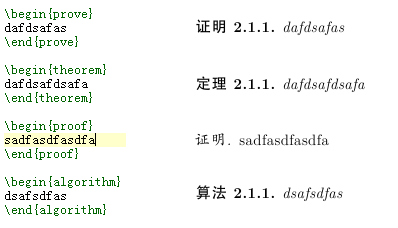
\includegraphics[scale=1]{figures/proofandprove}}
  \figcaption{proof、prove以及部分其他数学环境的差异}
  \label{pic:proofandprove}
\end{figure}

\section{使用模板的一些建议}

公式、章节、图和表格等(不包括脚注和参考文献)的交叉引用可以使用\verb|\autoref{label}|来得到正确的引用。例如使用\verb|\autoref{some_pic}|可以得到“图 X”的引用,使用\verb|\autoref{some_table}|可以得到“表 X”的引用。

建议使用\verb|\figcaption{}|命令得到所有图形的标题,表格也是。这样无论是否在图形环境中均能够得到正确的带图/表编号的标题,而在图形环境之外使用\verb|\caption{}|命令会报错。

%封面是按照制本厂的要求制作的,其中行宽和行高都是固定的,中文标题最多占两行,英文标题最多占三行。如果您的题目超过了这个限制,请缩减题目长度,不要擅自修改模板中的相关配置参数。


  %
\chapter{代码示例}
\label{chap:example}
\section{Euler数学字体示例}
$$
abcdefghijklmnopqrstuvwxyz
$$
$$
ABCDEFGHIJKLMNOPQRSTUVWXYZ
$$
$$
0123456789
$$
\begin{equation}
\begin{split}
\{S_i=0\}=\frac{a_i}{b_i+a_i} \\
\{S_i=1\}=\frac{b_i}{b_i+a_i} \label{1}
\end{split}
\end{equation}

\section{上标引用示例}
\verb|\scite{lshort-cn}|,效果\scite{lshort-cn}。

\section{表格环境加强命令示例}
本模板提供了表格环境下p\{width\}加强版命令,使用L\{width\}等可以在指定宽度的同时指定对齐方式。

\begin{minipage}{\textwidth}
\begin{Codex}[numbers=left]
\begin{table}
\tabcaption{几种命令效果对比的对比}
\label{tab:tblcmp}
\centering
\begin{tabular}{c||l|c|r|p{2.5cm}|L{2.5cm}|C{2.5cm}|R{2.5cm}}
\hline
命令&l&c&r&p\{width\}&L\{width\}&C\{width\}&R\{width\}\\
\hline
效果&左齐&居中&右齐&定宽&左齐定宽&居中定宽&右齐定宽\\
\hline
\end{tabular}
\end{table}
\end{Codex}

\tabcaption{几种命令效果对比的对比}
\label{tab:tblcmp}
\centering
\begin{tabular}{c||l|c|r|p{2.5cm}|L{2.5cm}|C{2.5cm}|R{2.5cm}}
\hline
命令&l&c&r&p\{width\}&L\{width\}&C\{width\}&R\{width\}\\
\hline
效果&左齐&居中&右齐&定宽&左齐定宽&居中定宽&右齐定宽\\
\hline
\end{tabular}
\end{minipage}

\section{自定义代码环境示例}
\label{codex}
\subsection{Code环境}
\begin{minipage}{\textwidth}
\begin{minipage}{0.4\textwidth}
\begin{Code}[label=a.cpp, numbers=left]
This is Code environment
A simple example.
For more options, see fancyvrb's manual.
\end{Code}
\end{minipage}
\hfill\begin{minipage}{0.4\textwidth}
\begin{Verbatim}[fontsize=\scriptsize,baselinestretch=0.9,xleftmargin=3mm,frame=lines,labelposition=all,framesep=5pt]
\begin{Code}[label=a.cpp, numbers=left]
This is Code environment
A simple example.
For more options, see fancyvrb's manual.
\end{Code}
\end{Verbatim}
\end{minipage}
\end{minipage}

\subsection{Codex环境}
\begin{minipage}{\textwidth}
\begin{minipage}{0.4\textwidth}
\begin{Codex}[label=a.cpp, numbers=left]
This is Codex environment
A simple example.
For more options, see fancyvrb's manual.
\end{Codex}
\end{minipage}
\hfill\begin{minipage}{0.4\textwidth}
\begin{Verbatim}[fontsize=\scriptsize,baselinestretch=0.9,xleftmargin=3mm,frame=lines,labelposition=all,framesep=5pt]
\begin{Codex}[label=a.cpp, numbers=left]
This is Codex environment
A simple example.
For more options, see fancyvrb's manual.
\end{Codex}
\end{Verbatim}
\end{minipage}
\end{minipage}

\subsection{CodeScript环境}
\begin{minipage}{\textwidth}
\begin{minipage}{0.4\textwidth}
\begin{CodeScript}[label=a.cpp, numbers=left]
This is CodeScript environment
A simple example.
For more options, see fancyvrb's manual.
\end{CodeScript}
\end{minipage}
\hfill\begin{minipage}{0.4\textwidth}
\begin{Verbatim}[fontsize=\scriptsize,baselinestretch=0.9,xleftmargin=3mm,frame=lines,labelposition=all,framesep=5pt]
\begin{CodeScript}[label=a.cpp, numbers=left]
This is CodeScript environment
A simple example.
For more options, see fancyvrb's manual.
\end{CodeScript}
\end{Verbatim}
\end{minipage}
\end{minipage}

\subsection{CodexScript环境}
\begin{minipage}{\textwidth}
\begin{minipage}{0.4\textwidth}
\begin{CodexScript}[label=a.cpp, numbers=left]
This is CodexScript environment
A simple example.
For more options, see fancyvrb's manual.
\end{CodexScript}
\end{minipage}
\hfill\begin{minipage}{0.4\textwidth}
\begin{Verbatim}[fontsize=\scriptsize,baselinestretch=0.9,xleftmargin=3mm,frame=lines,labelposition=all,framesep=5pt]
\begin{CodexScript}[label=a.cpp, numbers=left]
This is CodexScript environment
A simple example.
For more options, see fancyvrb's manual.
\end{CodexScript}
\end{Verbatim}
\end{minipage}
\end{minipage}

\section{表格示例}
具体代码请参考源文件./chapter/chap-example.tex。
\begin{table}[htbp]
\centering
\caption{基于因子分析的失配补偿结果}
\label{tab:jfa-gmm-ubm}
\begin{tabular}{cccccc}
    \toprule
    &\multirow{2}{*}{\#Mix}&\multicolumn{2}{c}{No-norm}
    &\multicolumn{2}{c}{Tnorm}\\
    \cline{3-4} \cline{5-6}
		&		& EER(\%) 	& MinDCF & EER(\%) 	& MinDCF\\
    \midrule
	\multirow{3}{*}{GMM-UBM}
    &256 		& 12.43 	& 0.0647	& 12.85    & 0.0580\\
    &512 		& 10.02 	& 0.0464	& 8.88 	   & 0.0370\\
    &1024 		& 9.97 	    & 0.0457	& 8.72 	   & 0.0372\\
    \midrule
	\multirow{3}{*}{Factor Analysis}
    &256 		& 8.09 	& 0.0331 	& 7.39 	& 0.0319\\
    &512 		& 7.08 	& 0.0305 	& 6.53 	& 0.0292\\
    &1024 		& 6.83 	& 0.0295 	& \textbf{6.29} 	& \textbf{0.0279}\\
 \bottomrule
\end{tabular}
\end{table}

\section{算法示例}
具体代码请参考源文件./chapter/chap-example.tex。
\IncMargin{1em}
\begin{algorithm}
\SetKwData{Left}{left}\SetKwData{This}{this}\SetKwData{Up}{up}
\SetKwFunction{Union}{Union}\SetKwFunction{FindCompress}{FindCompress}
\SetKwInOut{Input}{input}\SetKwInOut{Output}{output}
\Input{$O_t,UBM,U$}
\Output{$x,y$}
\BlankLine
\emph{$y\leftarrow 0;$$x_h\leftarrow 0;$$h=1,...,H$ }\;
\For{$i=1$ \KwTo Number of E-M iterations}{
\emph{E Step}:\\
\For{$h=1$ \KwTo $H$}{\label{forins}
对于每一条语音段,计算其EM统计量(零阶统计量$N_h$,一阶统计量$S_{X,h}$\;
}
计算每一个人所有语音段的零阶统计量$N$\\
计算每一个人所有语音段的一阶统计量$S$\\
\emph{M Step}:\\
\For{$j=1$ \KwTo Number of Gauss-Seidel iterations}{
\For{$h=1$ \KwTo $H$}{\label{forins}
估计每一语音段$h$的失配因子$x_h$
}
估计模型的话者因子$y$
}
}
\Return{$\mu = m+Dy$}
\caption{disjoint decomposition}\label{algo_disjdecomp}
\end{algorithm}\DecMargin{1em}

\section{引用参考文献示例}
参考文献测试:\citep{deng:01a}

  %自行添加
  %\include{chapter/...}

%%%%%%%%%%%%%%%%%%%%%%%%%%%%%%
%% 附件部分
%%%%%%%%%%%%%%%%%%%%%%%%%%%%%%
\backmatter

  % 参考文献
  % 使用 BibTeX
  % 选择参考文献的排版格式。注意ustcbib这个格式不保证完全符合要求,请自行决定是否使用
  \bibliographystyle{ustcbib}%{GBT7714-2005NLang-UTF8}
  \bibliography{bib/tex}
  \nocite{*} % for every item
  % 不使用 BibTeX
  % %\renewcommand{\baselinestretch}{0.5}
\begin{thebibliography}{10}

\bibitem{deng:01a}
{邓建松,~彭冉冉,~陈长松邓建松,~彭冉冉,~陈长松邓建松,~彭冉冉,~陈长松邓建松,~彭冉冉,~陈长松邓建松,~彭冉冉,~陈长松邓建松,~彭冉冉,~陈长松邓建松,~彭冉冉,~陈长松邓建松,~彭冉冉,~陈长松邓建松,~彭冉冉,~陈长松邓建松,~彭冉冉,~陈长松邓建松,~彭冉冉,~陈长松}.
\newblock {\em \LaTeXe{}~科技排版指南}.
\newblock 科学出版社,~书号:~7-03-009239-2/TP.1516, 北京, 2001.

\bibitem{wang:00a}
王磊.
\newblock {\em \LaTeXe{}~插图指南}.
\newblock 2000.

\bibitem{zhang:03a}
张林波.
\newblock {\em 关于新版~CCT~的说明}.
\newblock 2003.

\bibitem{lshort-cn}
C\TeX{} 翻译小组.
\newblock {\em lshort~中文版~3.20}.
\newblock 2003.

\bibitem{knuth86e}
Donald~E. Knuth.
\newblock {\em Computer Modern Typefaces}, volume~E of {\em Computers and
  Typesetting}.
\newblock Addison-Wesley, Reading, Massachusetts, 1986.

\bibitem{knuth86d}
Donald~E. Knuth.
\newblock {\em {METAFONT}: The Program}, volume~D of {\em Computers and
  Typesetting}.
\newblock Addison-Wesley, Reading, Massachusetts, 1986.

\bibitem{knuth86c}
Donald~E. Knuth.
\newblock {\em The {METAFONT}book}, volume~C of {\em Computers and
  Typesetting}.
\newblock Addison-Wesley, Reading, Massachusetts, 1986.

\bibitem{knuth86b}
Donald~E. Knuth.
\newblock {\em {TeX}: The Program}, volume~B of {\em Computers and
  Typesetting}.
\newblock Addison-Wesley, Reading, Massachusetts, 1986.

\bibitem{knuth86a}
Donald~E. Knuth.
\newblock {\em The {TeX}book}, volume~A of {\em Computers and Typesetting}.
\newblock Addison-Wesley, Reading, Massachusetts, 1986.

\bibitem{lamport85a}
Leslie Lamport.
\newblock {\em {LaTeX} --- A Document Preparation System: User's Guide and
  Reference Manual}.
\newblock Addison-Wesley, Reading, Massachusetts, 2nd edition, 1985.

\end{thebibliography}


  % 附录,没有请注释掉
  %\begin{appendix}
    %
\chapter{关于硕士、博士学位论文撰写要求}
\label{chap:requires}

学位论文是学位申请者为申请学位而撰写的学术论文,它集中作者在研究工作中获得可行的发明、理论和见解,是评判学位申请人学术水平的重要依据和获得学位的必要条件之一,也是科研领域中的主要文献资料和社会宝贵财富。
为提高研究生学位论文的质量,做到学位论文在内容和格式上规范化与统一化,特作如下规定:

\section{对学位论文的基本要求}

\textbf{一下文字仅作示例,一切以学校规定为准!}

\subsection{硕士学位论文}

根据《中华人民共和国学位条例暂行实施办法》第八条的规定,硕士学位论文应能表明作者确已在本门学科上掌握了坚实的基础理论和系统的专门知识,并对所研究的课题有新的见解,有从事科学研究或独立担负专门技术工作的能力。硕士学位论文工作一般是在硕士生完成培养计划规定的课程学习后开始,其工作内容因学科的性质不同而有所差异,一般包括文献阅读、开题报告、拟定并实施工作计划、科研调查、实验研究、理论分析和文字总结等工作。论文正文一般应不少于3万字。硕士学位论文必须有一定的工作量,在论文题目确定后,用于论文工作的时间一般不应少于1.5年。

\subsection{博士学位论文}

根据《中华人民共和国学位条例暂行实施办法》第十三条的规定,博士学位论文应能表明作者确已在本门学科上掌握了坚实宽广的基础理论和系统深入的专门知识,具有独立从事科学研究工作的能力,并在科学或专门技术工作上做出了创造性的成果。博士学位论文工作是攻读博士学位研究生培养的最重要环节,其工作时间一般应不少于2学年。博士生入学后在导师指导下明确科研方向,收集资料,阅读文献,进行调查研究,确定研究课题。一般在第二至第三学期通过开题报告并制定论文工作计划。博士生应根据论文工作计划分阶段在教研室、学术会议上报告科研和论文工作的进展情况。论文正文一般应不少于5万字。博士生用于论文研究和撰写学位论文的时间一般应不得少于2年。

特别应注意,学位论文应是本人的研究成果,在导师指导下独立完成,不得抄袭或剽窃他人成果。论文应反映作者较好地掌握了本学科、专业的研究方法和技能,学术观点必须言之有理、持之有据,论文内容应层次分明,数据可靠,文字简炼,推理严谨,立论正确。

\section{对学位论文的格式要求}

\subsection{编写要求}

硕士、博士学位论文一般应由以下全部或某几部分组成,依次为:封面、中文摘要、英文摘要 、目录、符号说明、正文、参考文献、附录、附图表、致谢、攻读学位期间发表的学术论文目录。

具体要求如下:

\subsubsection{封面}

采用研究生院规定的统一封面,封面上填写论文题目、作者姓名、导师姓名、学科(专业) 、论文完成时间。上述内容也应在扉页上填写清楚。论文题目采用黑体26磅加粗居中,其他采用宋体16磅居中。书脊用黑体12磅,上方写论文题目,中间写系别,下方写研究生姓名(彩色封面在制信厂或印刷厂装订)。

\subsubsection{论文摘要}

学位论文的中文摘要应以最简洁的语言介绍论文的概要、作者的突出论点、新见解或创造性成果。硕士学位论文中文摘要一般应在500字左右,博士学位论文中文摘要一般在1500字左右。英文摘要(Abstract)内容应与中文摘要基本相对应,要语句通顺,语法正确,能正确概括文章的内容。摘要标题采用黑体16磅居中,正文采用宋体12磅(英文用Times New Roman体12磅),行距20磅。

\subsubsection{正文}

正文是学位论文的主体和核心部分,它是将学习、研究和调查过程中筛选、观察和测试所获得的材料,经过加工整理和分析研究,由材料而形成论点。不同学科、专业有着不同的写作内容,但作为一般要求,论据、论点应力求准确、完备、清晰、通顺,实事求是,客观真切,简短精炼,合乎逻辑。一般标题字体采用黑体14磅,多级标题可采用粗体14磅或粗体12磅。正文字体采用宋体12磅(英文用Times New Roman体12磅),两端对齐书写,行距20磅。


绪论或引言是学位论文主体部分的开端,主要说明研究工作的缘起、沿革、目的、涉及范围 、国内外研究现状、相关领域的前人研究成果和知识空白、理论分析的依据、研究设想、研究方法和实际设计的概述,以及文中拟解决的问题、理论意义和实用价值等,应言简意赅,不要与摘要雷同或成为摘要的解释,也不是提要。

结论是学位论文最终和总体的结论,是整篇论文的归宿,应明确、精炼、完整、准确。要着重阐述作者研究的创造性成果、新见解、新发现和新发展,及其在本研究领域中的地位、作用、价值和意义,还可进一步提出需要讨论的问题和建议。学位论文中的计量单位、制图、制表、公式规范、缩略词和符号必须遵循GB 3100~3102—93(国家技术监督局1993-12-27发布,1994-07-01实施)有关量和单位的规定。如无标准可循,应采用本学科或专业有关权威性机构或学术团体所公布的规定。如不得已必需引用某些未公知公用的、不易为同行读者所理解的或系作者自行拟定的符合、记号、缩略词等,均应一一在第一次出现时加以说明,给以明确的定义。

\subsubsection{参考文献}

参考文献应按文中引用的顺序列出,可以分列在各章末尾,也可以列在正文的末尾。

本着以严谨求实的科学态度撰写论文,凡学位论文中有引用他人成果之处,均应详细列出所引文献的名称、作者、发表刊物、发表时间、卷号、页码等。标题字体采用黑体14磅,正文字体采用宋体10磅(英文用Times New Roman体10磅),行距16磅。

\subsubsection{附录}
主要列入正文内过分冗长的公式推导,供查读方便所需的辅助性数学工具或表格,重复性数据图表,论文使用的缩写,程序全文及说明等。

\subsubsection{致谢}

表达作者对完成论文和学业提供帮助的老师、同学、领导、同事及亲属的感激之情。

\subsubsection{攻读学位期间发表的学术论文目录}

按学术论文发表的时间顺序,列齐本人在攻读学位期间发表或已录用的学术论文清单(发表刊物名称、卷册号、页码、年月及论文署名、作者排序)。

\subsection{打印}

按照有关规定,凡授予中华人民共和国学位者,学位论文必须用中文撰写,同时一律用A4标准纸打印输出,一般应有篇眉。篇眉和页码均采用宋体10磅居中,页面设置上边距3.8cm、下边距为3.0cm,左边距为3.5cm、右边距为3.0cm。

\subsection{装订}

学位论文撰写完成后,用研究生院统一封面线装订成册。所需份数由研究生本人及导师掌握(可参考学位申请上报材料清单的要求)。

  %\end{appendix}

  \makeatletter
  \ifustc@bachelor\relax\else
    % 致谢
	
\begin{thanks}
为期三年的研究生生活即将结束,此时此刻,心中充满了感激和不舍。

首先我要感谢我的导师唐珂老师,他待人和善,学识渊博,工作一丝不苟,无论在工作中还是生活上,都给予了我莫大的帮助。
很荣幸能在这样优秀的导师指导下,开展和完成我的研究工作。

我要感谢实验室的各位同门,在这三年中,与大家相处得非常融洽,在紧张充实的学习之余,大家也会经常一起组织各种娱乐活动,与大家相处总是少不了欢乐。

我要感谢在这篇毕业论文成文期间,好友姚亚强,实验室魏语凡、姜春晖、谢格、李皈颖、钟锦红等同学的帮助,没有你们,我无法这么快完成论文的写作工作。

我要感谢我的父母,感谢他们在我这段求学经历中所给予的无微不至的关怀和精神上的无条件支持,他们是我最坚实的后盾,无论走到哪里,想到他们就无比的温暖和感激。

最后衷心感谢各位论文评审老师耐心地审阅我的论文并提出宝贵的意见。
%\vskip 18pt
\begin{flushright}
沈汪洋

\today
\end{flushright}

\end{thanks}
%硕博致谢部分
    % 发表文章目录
    
\chapter{在读期间发表的学术论文与取得的研究成果}

\noindent\textbf{研究工作:}

\begin{enumerate}

\item A A A A A A A A A
\item A A A A A A A A A
\item A A A A A A A A A
\item A A A A A A A A A

\end{enumerate}


\noindent\textbf{已发表论文:}

\begin{enumerate}

\item A A A A A A A A A 
\item A A A A A A A A A
\item A A A A A A A A A
\item A A A A A A A A A
\item A A A A A A A A A
\item A A A A A A A A A
\item A A A A A A A A A
\item A A A A A A A A A

\end{enumerate}

\vskip 1cm

\noindent\textbf{待发表论文:}

\begin{enumerate}

\item A A A A A A A A A

\end{enumerate} 
  \fi
  \makeatother

\end{document}
